\section{Mạch xác lập điều hòa}
\subsection{Quá trình tuần hoàn}
Tín hiệu khảo sát: dòng điện $i(t)$, điện áp $u(t)$. Tuần hoàn $f(t) = f(t+T)$.

\textbf{Trị hiệu dụng:}
\begin{itemize}
    \item Dòng điện (điệnáp) tuần hoàn sẽ có trị hiệu dụng $I_{RMS} \ (U_{RMS})$ là bằng với trị số dòng (áp) DC khi công suất tiêu tán trung bình do 2 dòng điện (điện áp) gây ra trên cùng điện trở R là như nhau.
    \item Biểu thức tính trị hiệu dụng (RMS - Root Mean Square).
\end{itemize}
\begin{equation}
    I_{RMS} = \sqrt{\frac{1}{T} \int_{1}^{T} i^2(t)dt} \qquad \qquad U_{RMS} = \sqrt{\frac{1}{T} \int_{1}^{T} u^2(t)dt}
\end{equation}
\subsection{Quá trình điều hòa}
\begin{itemize}
    \item Dòng điện, điện áp:
        \[
            i(t) = I_m \sin (\omega t + \varphi)
        \]
        \[
            u(t) = U_m \sin (\omega t + \Psi)
        \]
    \item $I_m, \ U_m$: biên độ, $\omega:$ tần số góc, $\varphi, \Psi:$ pha ban đầu.
\end{itemize}
\begin{center}
    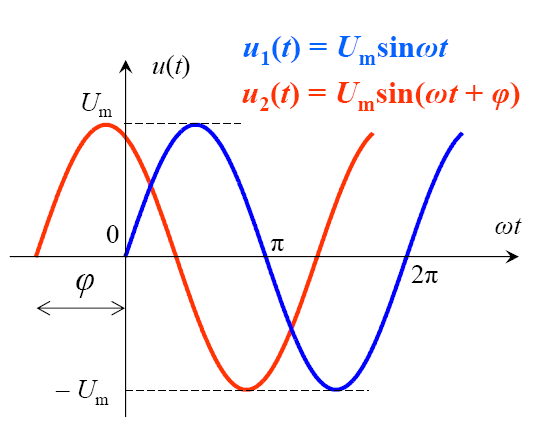
\includegraphics[width = 0.5\textwidth]{./image/29.png}
\end{center}
\begin{itemize}
    \item $\varphi:$ pha ban đầu, ta có thể nói $u_2(t)$ sớm pha so với $u_1(t)$ hoặc $u_1(t)$ chậm pha so với $u_2(t)$.
    \item $\varphi \neq 0,$ ta nói $u_1(t)$ và $u_2(t)$ lệch pha.
    \item $\varphi = 0,$ ta nói $u_1(t)$ và $u_2(t)$ đồng pha.
\end{itemize}
\textbf{So sánh pha hai tín hiệu điều hòa:}
\begin{itemize}
    \item Cùng tần số.
    \item Cùng dạng lượng giác.
    \item Cùng dạng biên độ (cực đại hay hiệu dụng).
\end{itemize}

Ta nói $u_1(t)$ nhanh pha hơn $u_2(t)$ một góc $\varphi$ thì $\varphi=\varphi_1 - \varphi_2$ (hay ta có thể nói $\varphi_2$ chậm pha hơn $\varphi_1$ một góc $\varphi$). Nếu ta nói $u_2(t)$ nhanh pha hơn $u_1(t)$ một góc $\varphi$ thì $\varphi=\varphi_2 - \varphi_1$.
\subsection{Phương pháp biên độ phức}
\[
    u(t) = U_m \sin (\omega t  + \varphi)
\]
\begin{center}
    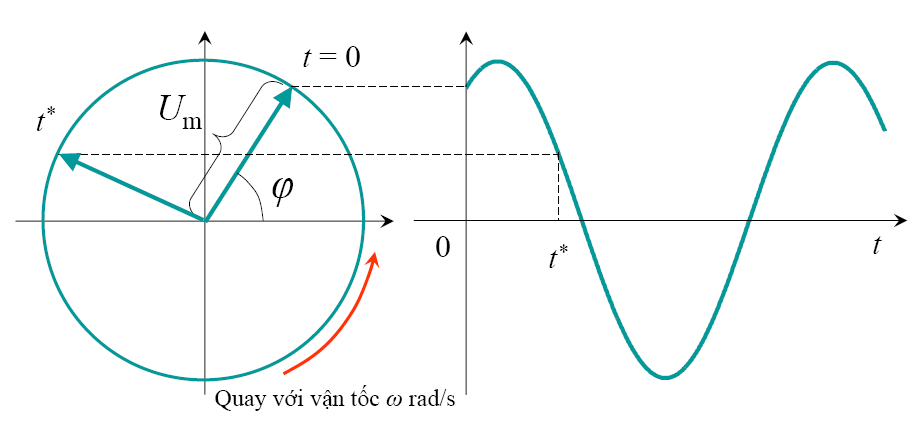
\includegraphics[width = 0.8\textwidth]{./image/30.png}
\end{center}
\textbf{Vector quay.}
\begin{center}
    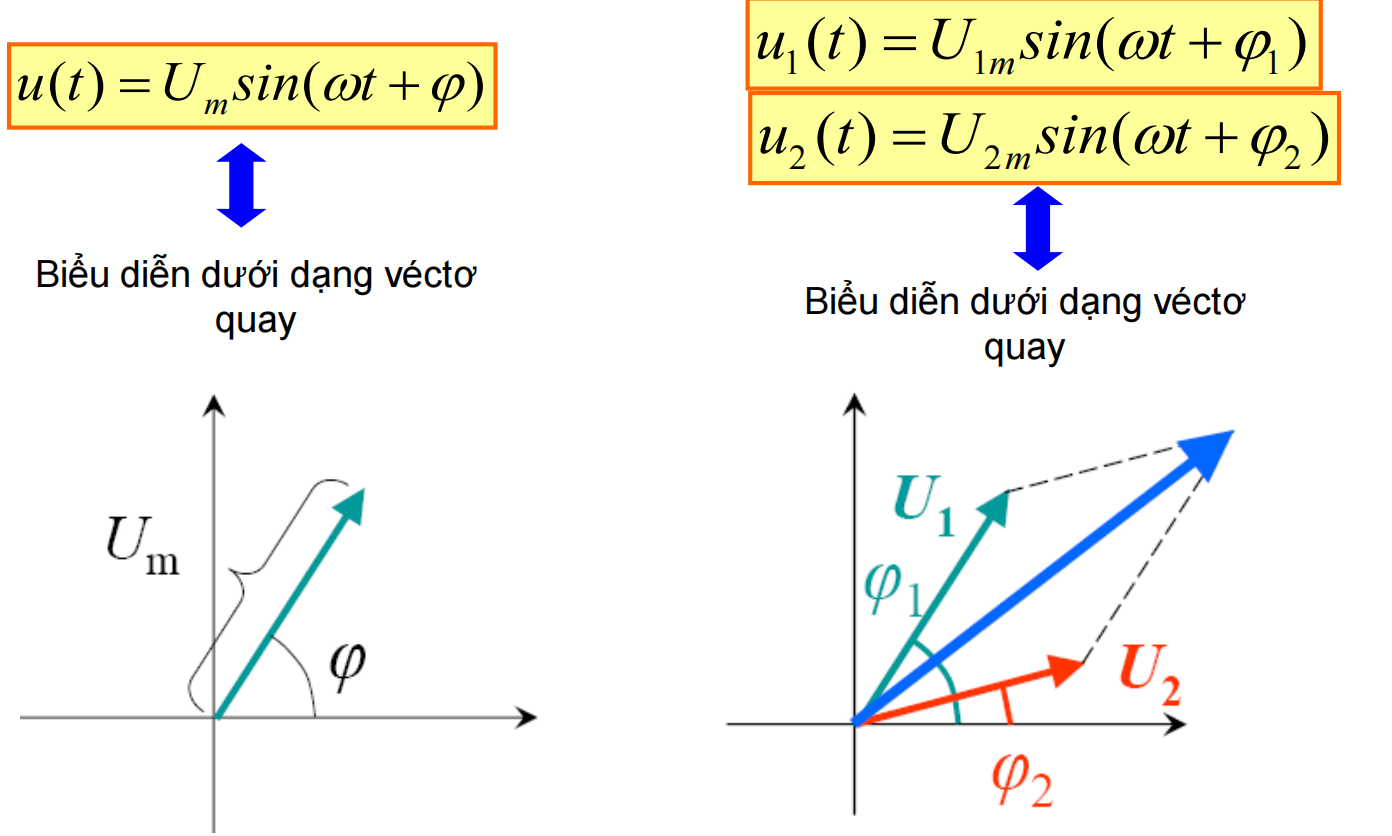
\includegraphics[width = 0.8\textwidth]{./image/31+32.png}
\end{center}
\begin{center}
    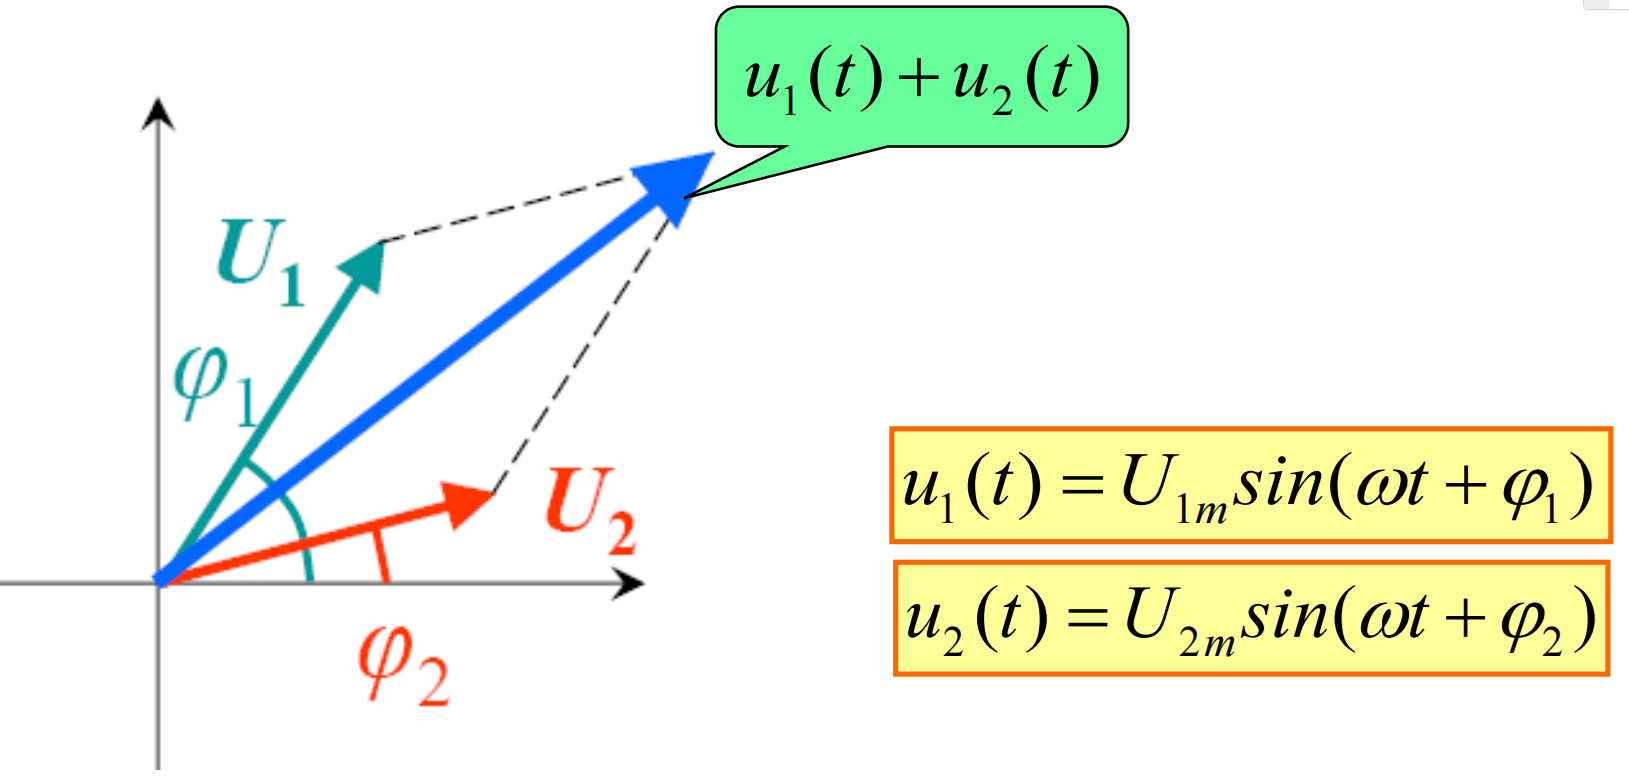
\includegraphics[width = 0.8\textwidth]{./image/33.png}
\end{center}
\[
    \begin{aligned}
        u(t) &= u_1(t) + u_2(t)\\
             &= U_{1m}\sin(\omega t + \varphi_1) + U_{2m}\sin(\omega t + \varphi_2)
    \end{aligned}
\]
\textbf{Ảnh phức.}

\textit{\textbf{Ảnh phức cho tín hiệu điều hòa}}
\begin{center}
    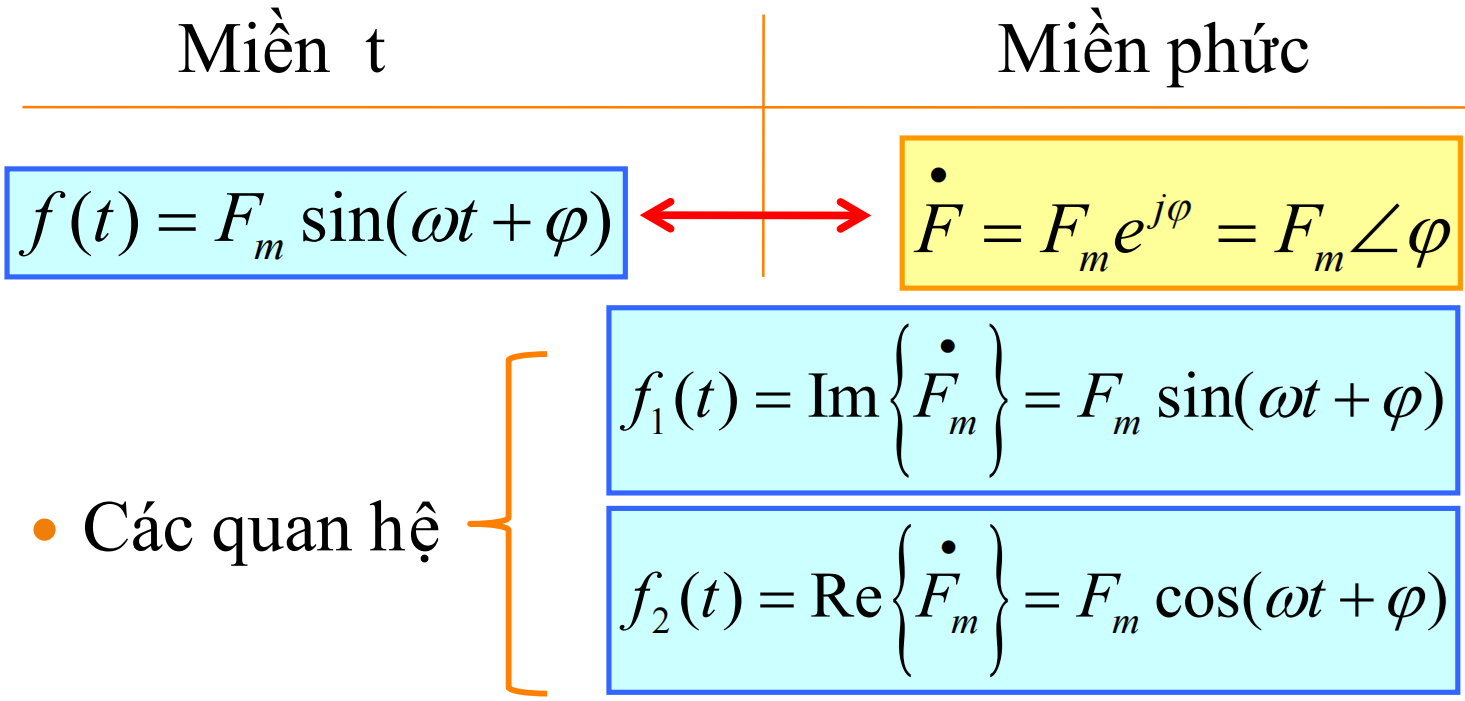
\includegraphics[width = 0.8\textwidth]{./image/34.png}
\end{center}

\textit{\textbf{Hiệu dụng phức:}} $\dot{F_{RMS}} = \dfrac{\dot{F}}{\sqrt{2}}$\\
\textbf{Các tính chất của vector biên độ phức.}

Cho $ f(t) \longleftrightarrow \dot F;\  g(t) \longleftrightarrow \dot G$.
\[
    f(t) = 3\cos (2t + 30^o) \Leftrightarrow \dot F = 3 \angle 30^o
\]
\[
    g(t) = 4\cos(2t - 60^o )\Leftrightarrow \dot G = 4 \angle -60^o
\]
\begin{itemize}
    \item Tính tỉ lệ: $kf(t) \Leftrightarrow k\dot F$
        \[
            3f(t) \Leftrightarrow 3\dot F = 9 \angle 30^o
        \]
    \item Tính xếp chồng: $f(t) \pm g(t) \Leftrightarrow \dot F \pm \dot G$
    \[
        f(t) + g(t) \Leftrightarrow \dot F + \dot G = 3 \angle 30^o + 4 \angle -60^o = 5 \angle -23,13^o = 5\cos (2t - 23,13^o)
    \]
    \item Tính đạo hàm: $\dfrac{df(t)}{dt} \Leftrightarrow j \omega \dot{F}$
        \[
            \frac{df(t)}{dt} = -6\sin (2t + 30^o) = 6\cos (2t+120^o) \Leftrightarrow j2\dot{F} = 6\angle 120^o
        \]
    \item Tính tích phân: $\displaystyle \int f(t)dt \Leftrightarrow \frac{1}{j\omega}\dot{F}$
        \[
            \int f(t)dt = \frac{3}{2}\sin (2t+30^o) = \frac{3}{2}\cos(2t-60^o) \Leftrightarrow \frac{1}{j2}\dot{F} = \frac{3}{2}\angle -60^o
        \]
\end{itemize}
\subsection{Giải bài toán mạch dùng ảnh phức}
\textbf{Phương pháp vector biên độ phức}
\begin{center}
    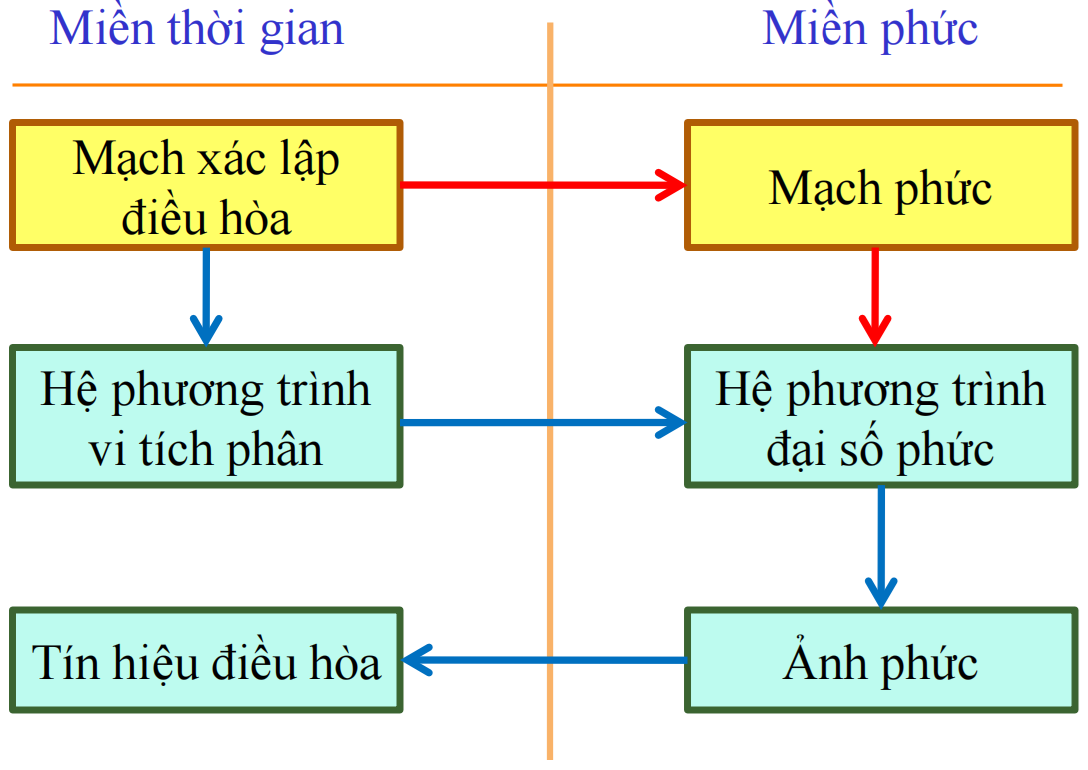
\includegraphics[width = 0.7\textwidth]{./image/36.png}
\end{center}
\subsection{Quan hệ dòng áp trên các phần tử mạch}
\subsubsection{Điện trở}
\begin{center}
    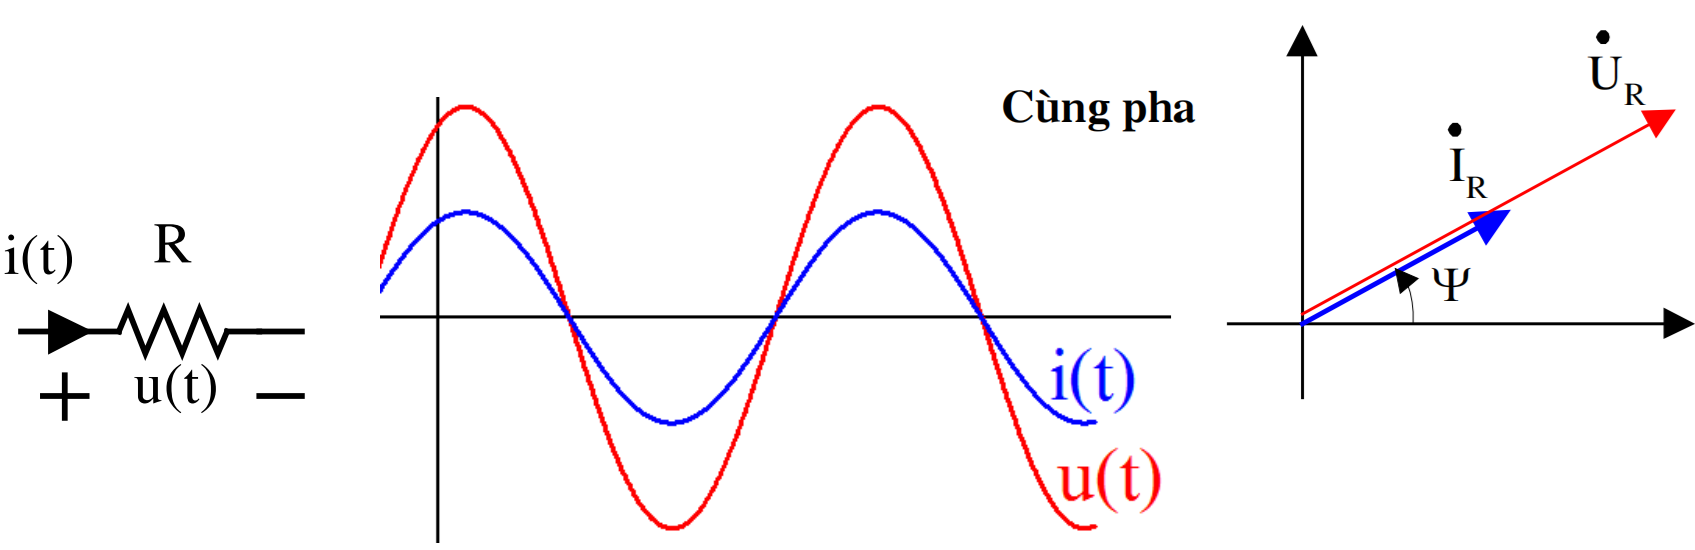
\includegraphics[width = 0.8\textwidth]{./image/37.png}
\end{center}
\begin{equation}
    i_R = I_m \cos (\omega t + \varPsi) \Leftrightarrow \dot{I_R} = I_m \angle \varPsi
\end{equation}
\begin{equation}
    u_R = Ri_R = RI_m (\omega t + \varPsi) \Leftrightarrow \dot{U_R} = RI_m \angle \varPsi
\end{equation}
Miền phức:
\begin{center}
    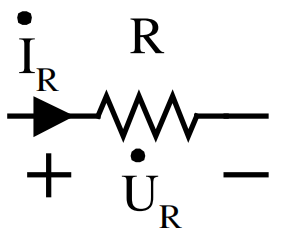
\includegraphics[width = 0.2\textwidth]{./image/38.png}
\end{center}
\begin{equation}
    \dot{U_R} = R\dot{I_R}
\end{equation}
\subsubsection{Điện cảm}
\begin{center}
    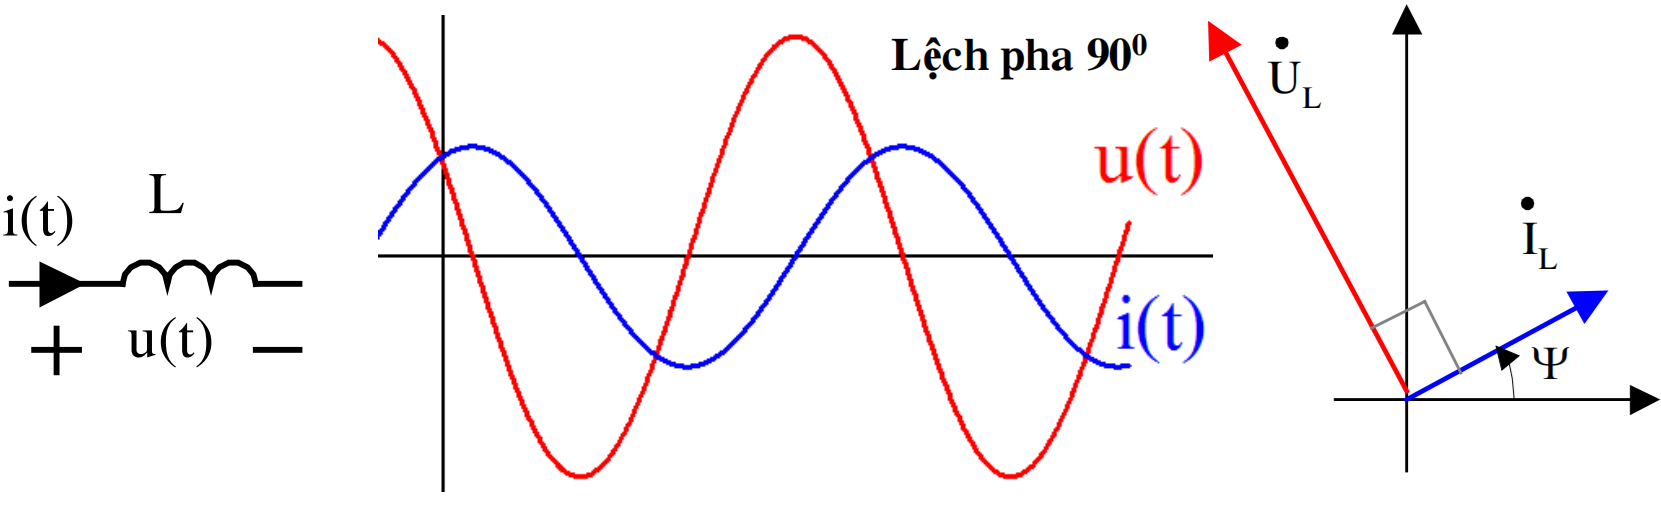
\includegraphics[width = 0.8\textwidth]{./image/39.png}
\end{center}
\begin{equation}
    i_L = I_m \cos (\omega t + \varPsi) \Leftrightarrow \dot{I_L} = I_m \angle \varPsi
\end{equation}
\begin{equation}
    u_L = L \frac{di_L}{dt} = \omega L I_m \cos (\omega t + \varPsi + 90^o) \Leftrightarrow \dot{U_L} = j\omega L I_m \angle \varPsi
\end{equation}
Miền phức:
\begin{center}
    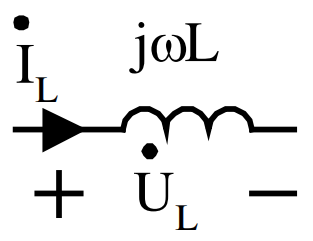
\includegraphics[width = 0.2\textwidth]{./image/40.png}
\end{center}
\begin{equation}
    \dot{U_L} = j\omega L \dot{I_L}
\end{equation}
\subsubsection{Điện dung}
\begin{center}
    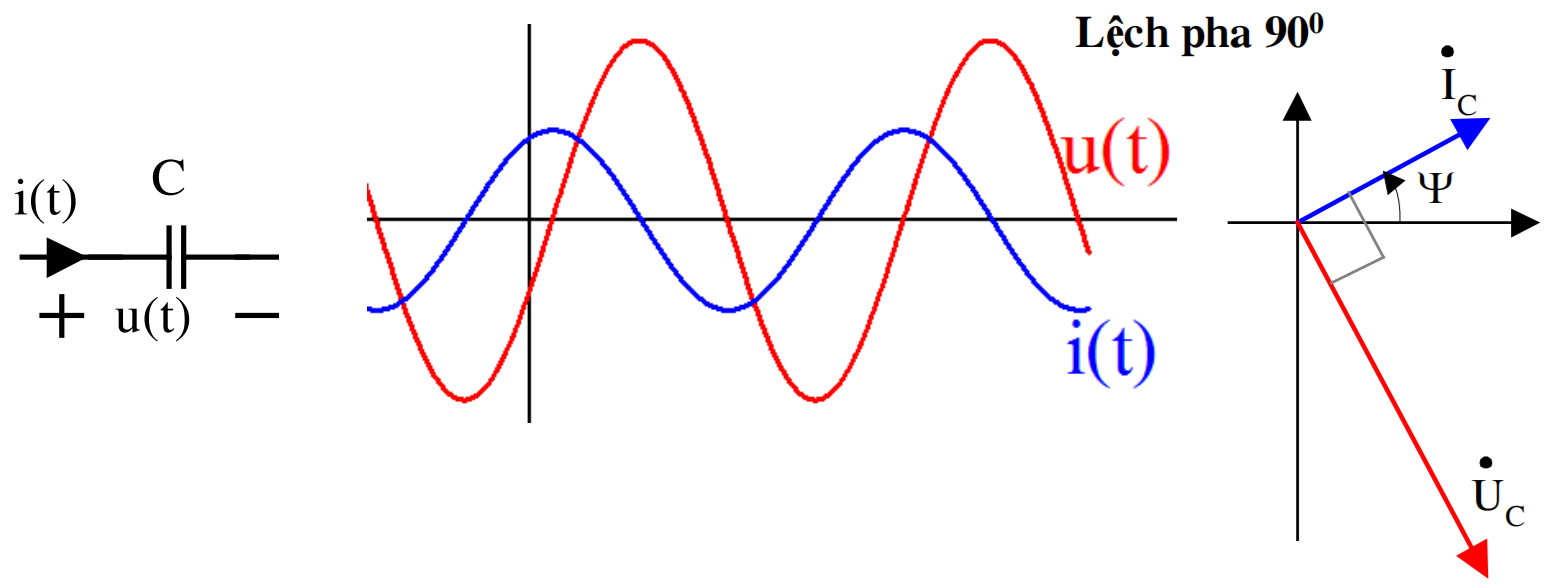
\includegraphics[width = 0.8\textwidth]{./image/41.png}
\end{center}
\begin{equation}
    u_C = U_m \cos (\omega t + \varPsi) \Leftrightarrow \dot{U_C} = U_m \angle \varPsi
\end{equation}
\begin{equation}
    i_C = C \frac{du_C}{dt} = \omega C U_m \cos (\omega t + \varPsi + 90^o) \Leftrightarrow \dot{I_C} = j\omega C U_m \angle \varPsi
\end{equation}
Miền phức:
\begin{center}
    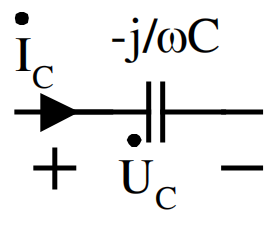
\includegraphics[width = 0.2\textwidth]{./image/42.png}
\end{center}
\begin{equation}
    \dot{U_C} = \frac{-j}{\omega C} \dot{I_C}
\end{equation}
\subsection{Các định luật dạng mạch phức}
\begin{center}
    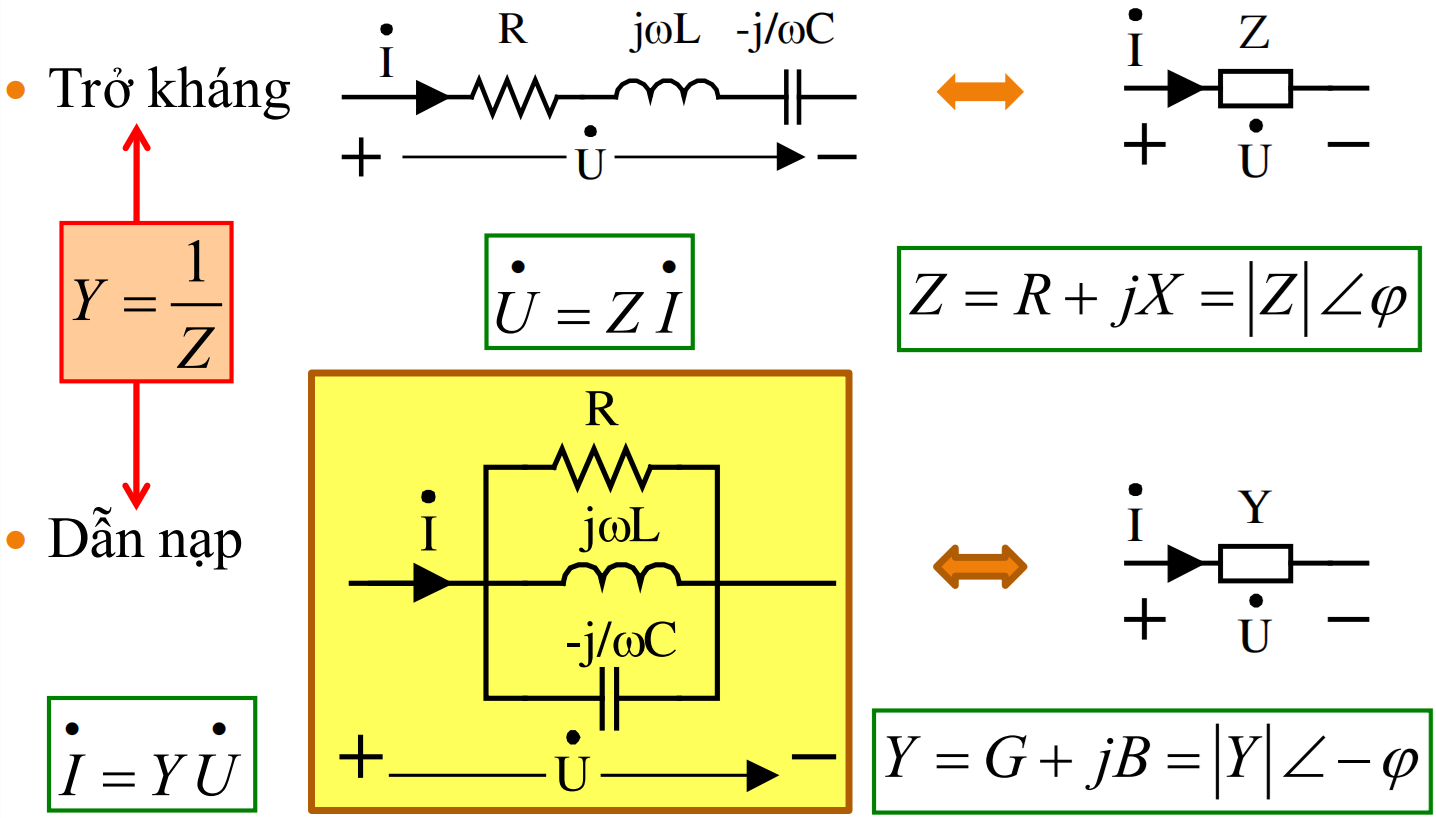
\includegraphics[width = 0.8\textwidth]{./image/43.png}
\end{center}
\subsubsection{Trở kháng $\&$ Dẫn nạp}
\begin{itemize}
    \item Z: Trở kháng, R: Điện trở, X: Điện kháng, Đơn vị tính: $\lbrack \Omega \rbrack$
         \begin{equation}
            Z = R + jX = |Z| \angle \varphi
         \end{equation}
        \begin{center}
            $|Z|$: module của Z \\
            $\varphi$: góc lệch pha giữa u và i
        \end{center}
    \item Y: Dẫn nạp, G: Điện dẫn, B: Điện nạp, Đơn vị tính: $\lbrack S \rbrack$
        \begin{equation}
             Y = G + jB = |Y| \angle -\varphi 
        \end{equation}
        \begin{center}
            $|Y|$: module của Y \\
            $-\varphi$: góc lệch pha giữa i và u
        \end{center}
\end{itemize}
\subsubsection{Định luật Kirchhoff dạng phức}
\begin{itemize}
    \item Định luật Kirchhoff dạng phức về dòng: Tổng các dòng điện phức tại một nút bằng không. Qui ước dòng đi vào nút mang dấu dương, đi ra nút mang dấu âm.
        \begin{equation}
            \sum_{\text{nút}}^{} \pm \dot{I}_K = 0
        \end{equation}
    \item Định luật Kirchhoff dạng phức về áp: Tổng các áp phức trong một vòng kín bằng không.
    \begin{equation}
        \sum_{\text{vòng kín}}^{} \pm \dot{U}_K = 0
    \end{equation}
\end{itemize}
\subsection{Công suất}
Xét một đoạn mạch mà dòng và áp tại xác lập điều hòa là:
\begin{equation}
    \vcenter{\hbox{\begin{minipage}{5cm}
    \centering
    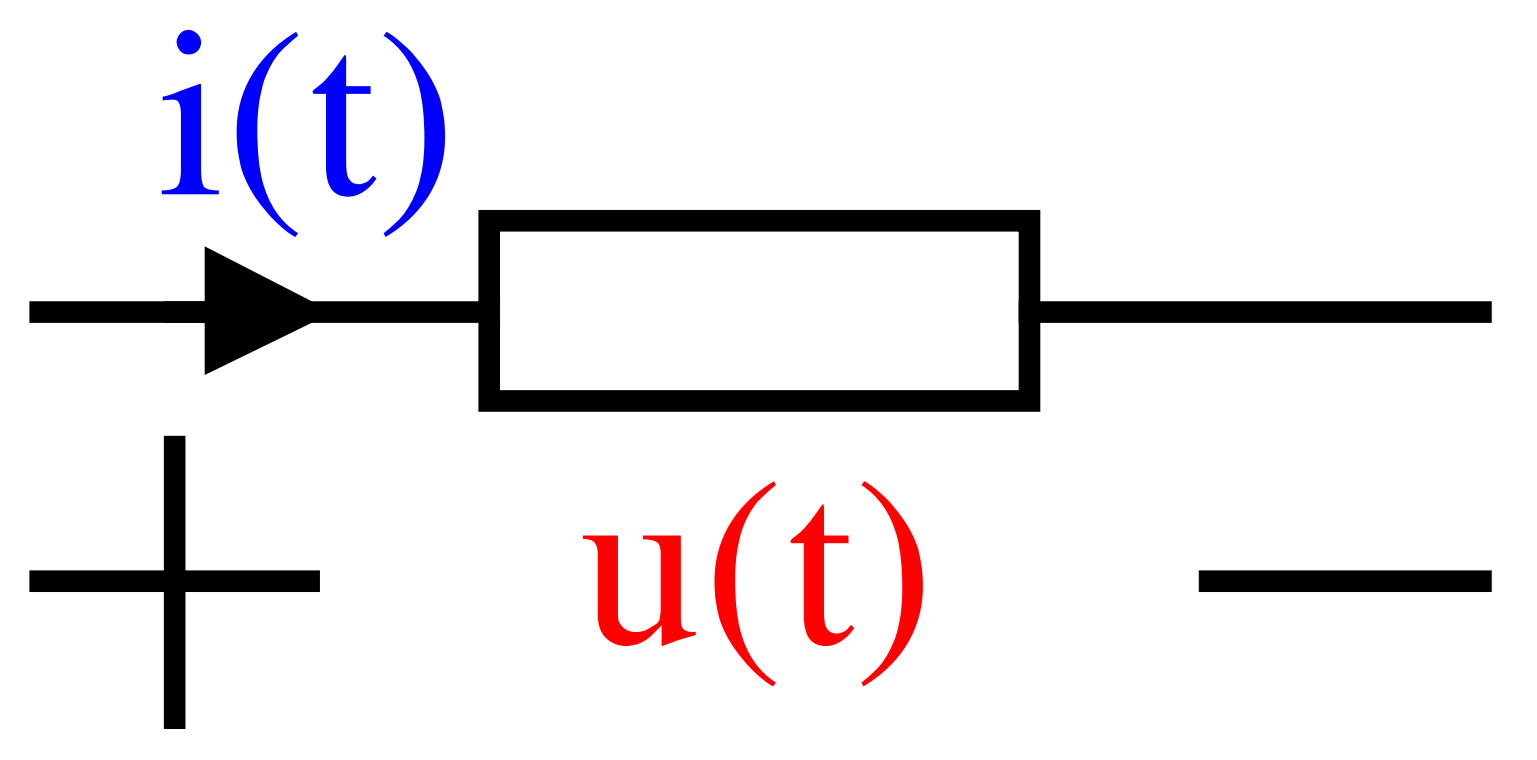
\includegraphics[width = 0.8\textwidth]{./image/44.png}
    \end{minipage}}}
    \qquad
    \begin{aligned}
        i(t) &= I_m\cos(\omega t + \varphi_i) \\
        u(t) &= U_m\cos(\omega t + \varphi_u)
    \end{aligned}
\end{equation}
Công suất tức thời
\begin{equation}
    p(t) = u(t)i(t) = \frac{1}{2}U_m I_m \cos (\varphi_u - \varphi_i) + \frac{1}{2}U_m I_m \cos(2\omega t + \varphi_u + \varphi_i)
\end{equation}
\begin{itemize}
    \item $p(t)>0$: mạch đang nhận công suất.
    \item $p(t)<0$: mạch đang phát công suất.
\end{itemize}
\begin{center}
    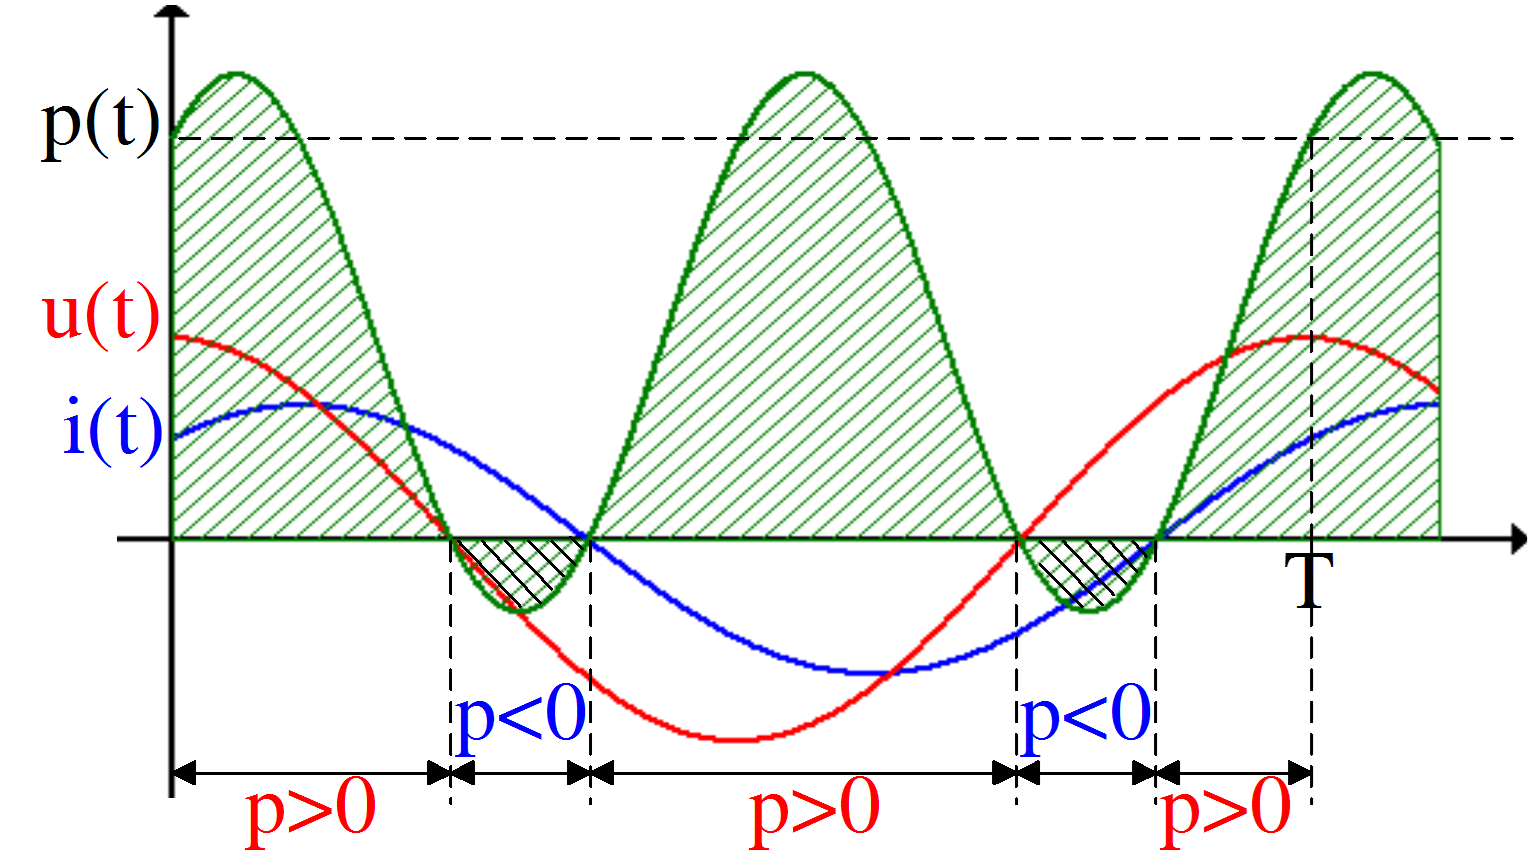
\includegraphics[width = 0.8\textwidth]{./image/45.png}
\end{center}
\subsubsection{Công suất tác dụng $\&$ Công suất phản kháng}
\begin{equation}
    \vcenter{\hbox{\begin{minipage}{5cm}
    \centering
    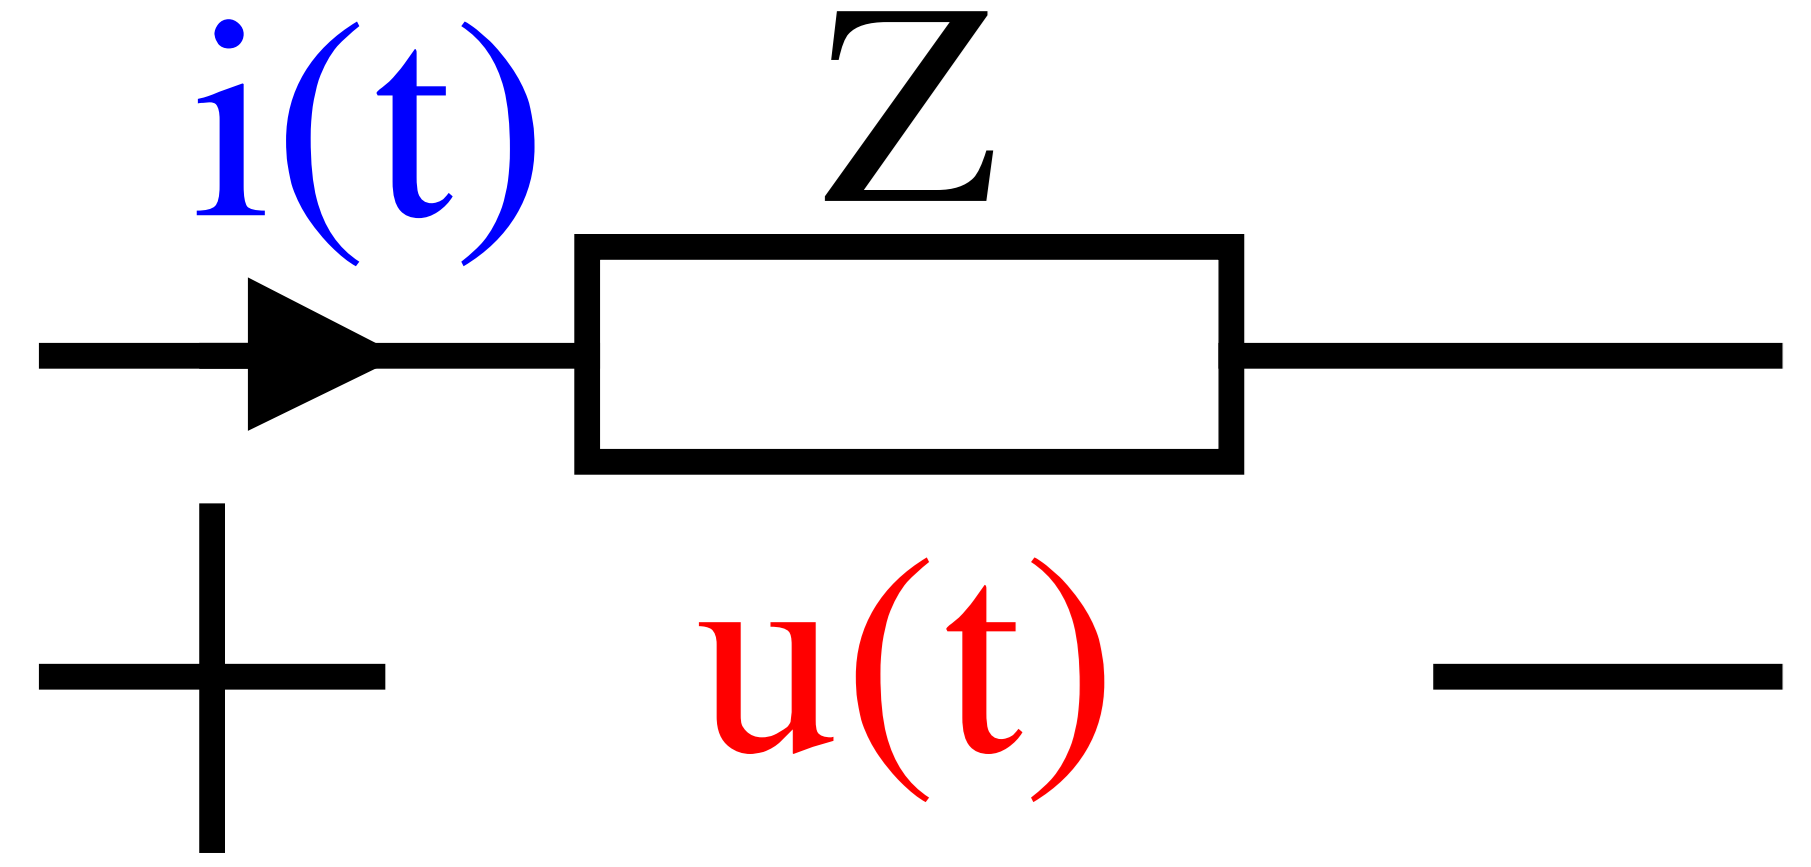
\includegraphics[width = 0.8\textwidth]{./image/46.png}
    \end{minipage}}}
    \qquad
    \begin{aligned}
        i(t) &= I_m\cos(\omega t + \varphi_i) \\
        u(t) &= U_m\cos(\omega t + \varphi_u) \\
        \varphi = \varphi_u - \varphi_i;\ Z = |Z| \angle \varphi
    \end{aligned}
\end{equation}
P (Active Power) $\lbrack W \rbrack$
\begin{equation}
    P = \frac{1}{T} \int_{t_0}^{t_0 + T} p(t)dt = \frac{1}{2}U_m I_m \cos \varphi \ \lbrack W \rbrack
\end{equation}
\begin{empheq}[box=\widefbox]{align}
    P &= UI \cos \varphi \\
    P &= \frac{1}{2} \text{Re} \lbrace \dot{U_m} I_m^\ast \rbrace \\
    P &= \frac{1}{2} I^2_m \text{Re} \lbrack Z \rbrack  \\
    P &= \frac{1}{2}U_m I_m \cos \varphi
\end{empheq}
Q (Reactive Power) $\lbrack VAr \rbrack$
\begin{empheq}[box=\widefbox]{align}
    Q &= UI \sin \varphi \\
    Q &= \frac{1}{2} \text{Im} \lbrace \dot{U_m} I_m^\ast \rbrace \\
    Q &= \frac{1}{2} I^2_m \text{Im} \lbrack Z \rbrack  \\
    Q &= \frac{1}{2}U_m I_m \sin \varphi
\end{empheq}
\subsubsection{Công suất trên các phần tử mạch}
\textbf{\textit{Điện trở:}}
\begin{center}
    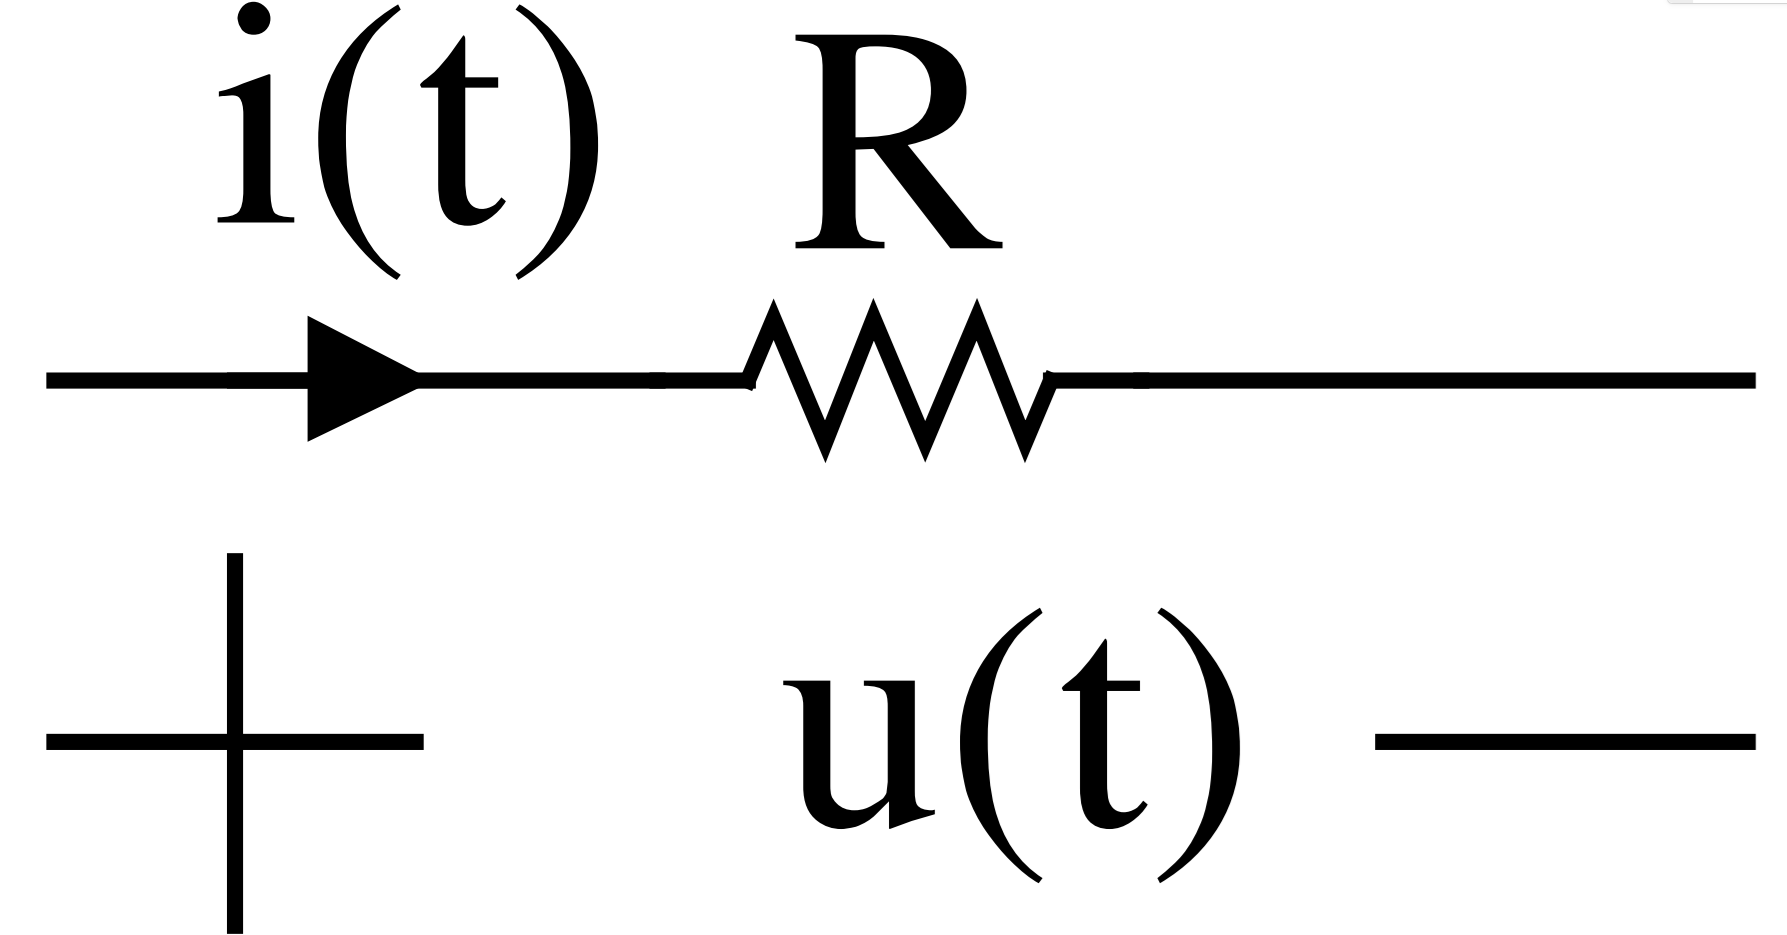
\includegraphics[width = 0.3\textwidth]{./image/48.png} \qquad 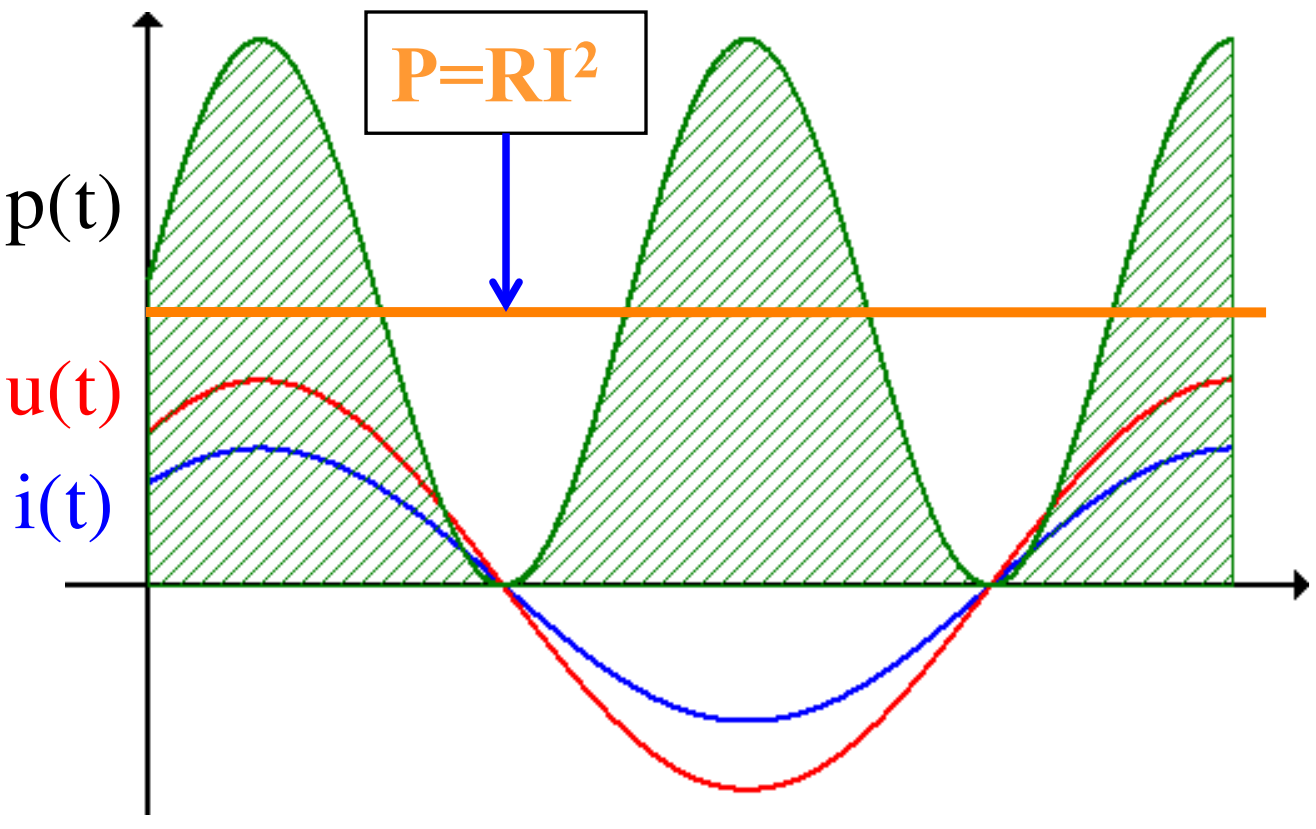
\includegraphics[width = 0.5\textwidth]{./image/47.png}
\end{center}
\begin{equation}
    i = I_m \cos (\omega t + \varPsi),\ u = Ri
\end{equation}
\begin{equation}
    p(t) = u(t)i(t) = Ri^2 = RI^2_m \cos^2 (\omega t + \varPsi) = \frac{1}{2}RI^2_m \lbrack 1 + \cos(2\omega t + 2\varPsi) \rbrack
\end{equation}
\begin{empheq}[box=\widefbox]{align}
    P &= \frac{1}{2}RI^2_m \\
    P &= RI^2 \\
    Q &= 0
\end{empheq}
\textbf{\textit{Điện cảm:}}
\begin{center}
    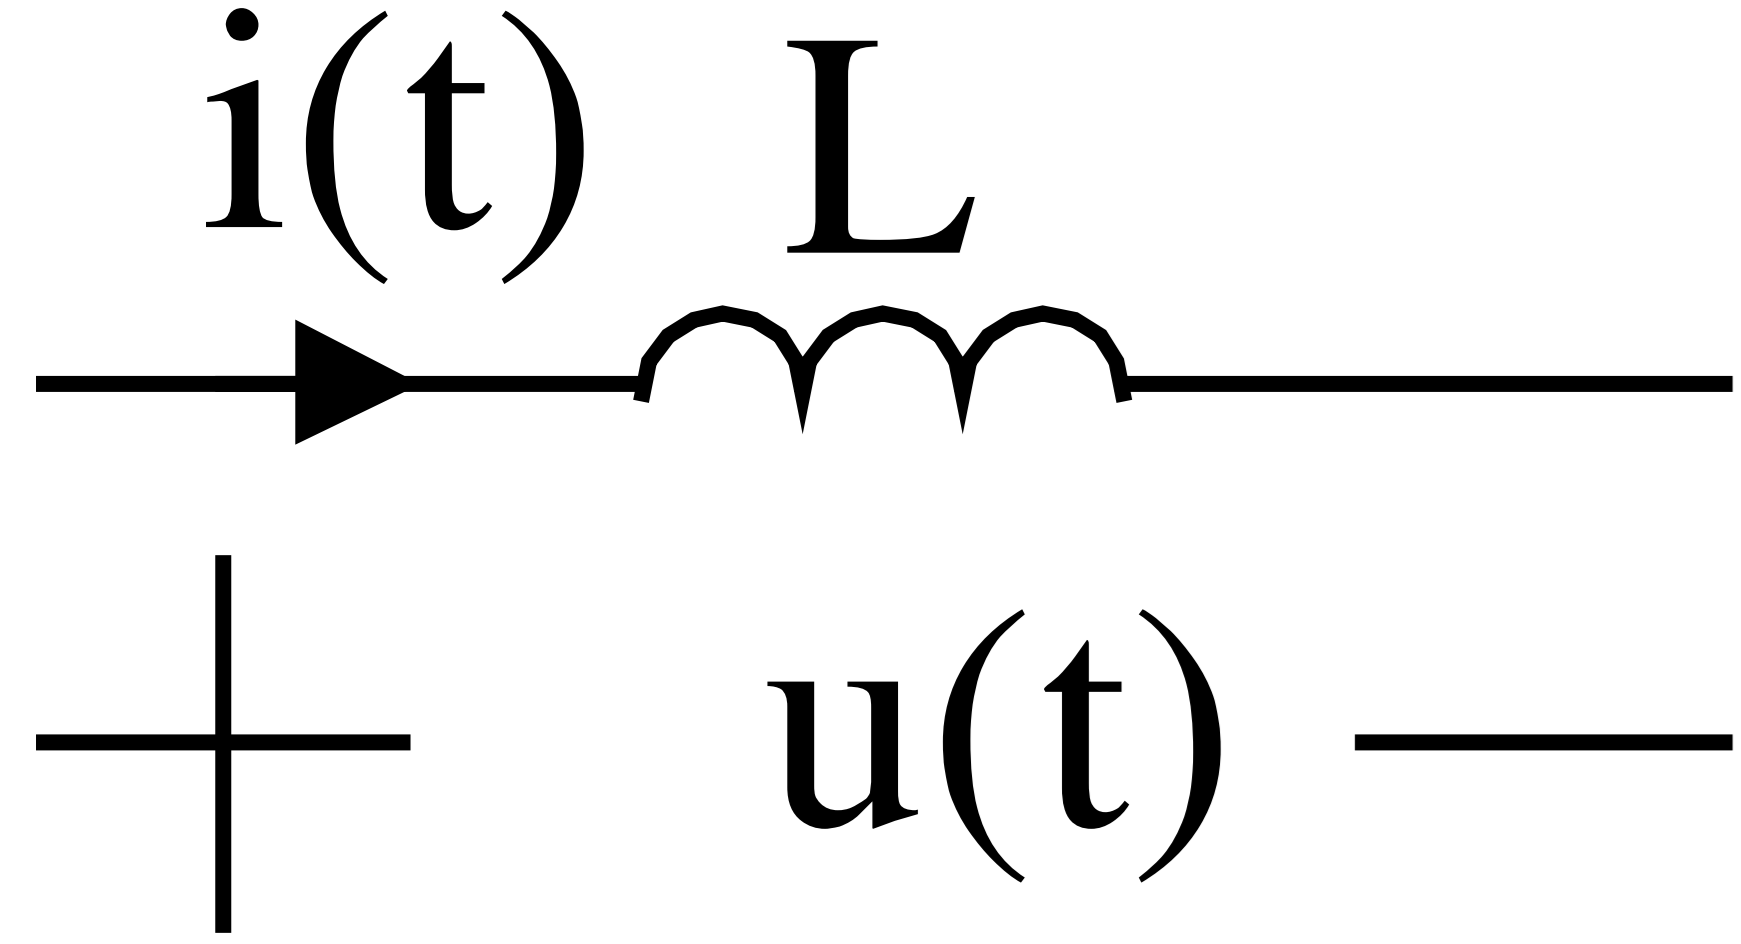
\includegraphics[width = 0.3\textwidth]{./image/49.png} \qquad 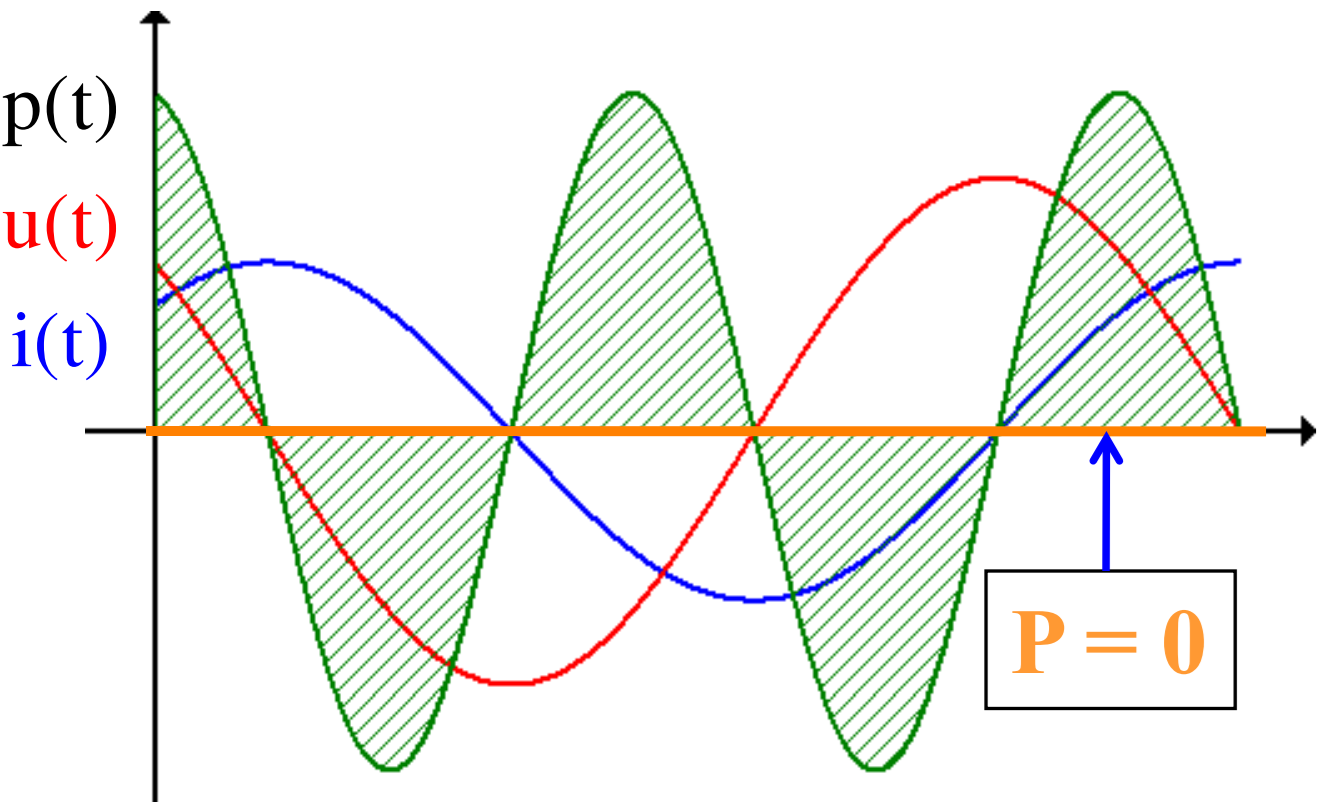
\includegraphics[width = 0.5\textwidth]{./image/50.png}
\end{center}
\begin{equation}
    i = I_m \cos (\Omega t + \varPsi),\ u = L\frac{di}{dt}
\end{equation}
\begin{equation}
    p(t) = u(t)i(t) = Li\frac{di}{dt} = -\omega LI^2_m \cos (\omega t + \varPsi) \sin (\omega t + \varPsi) = -\frac{1}{2}X_L I^2_m \sin (2\omega t + 2\varPsi) 
\end{equation}
\begin{empheq}[box=\widefbox]{align}
    P &= 0 \\
    Q &= \frac{1}{2}\omega LI^2_m \\
    Q &= 0
\end{empheq}
\textbf{\textit{Điện dung:}}
\begin{center}
    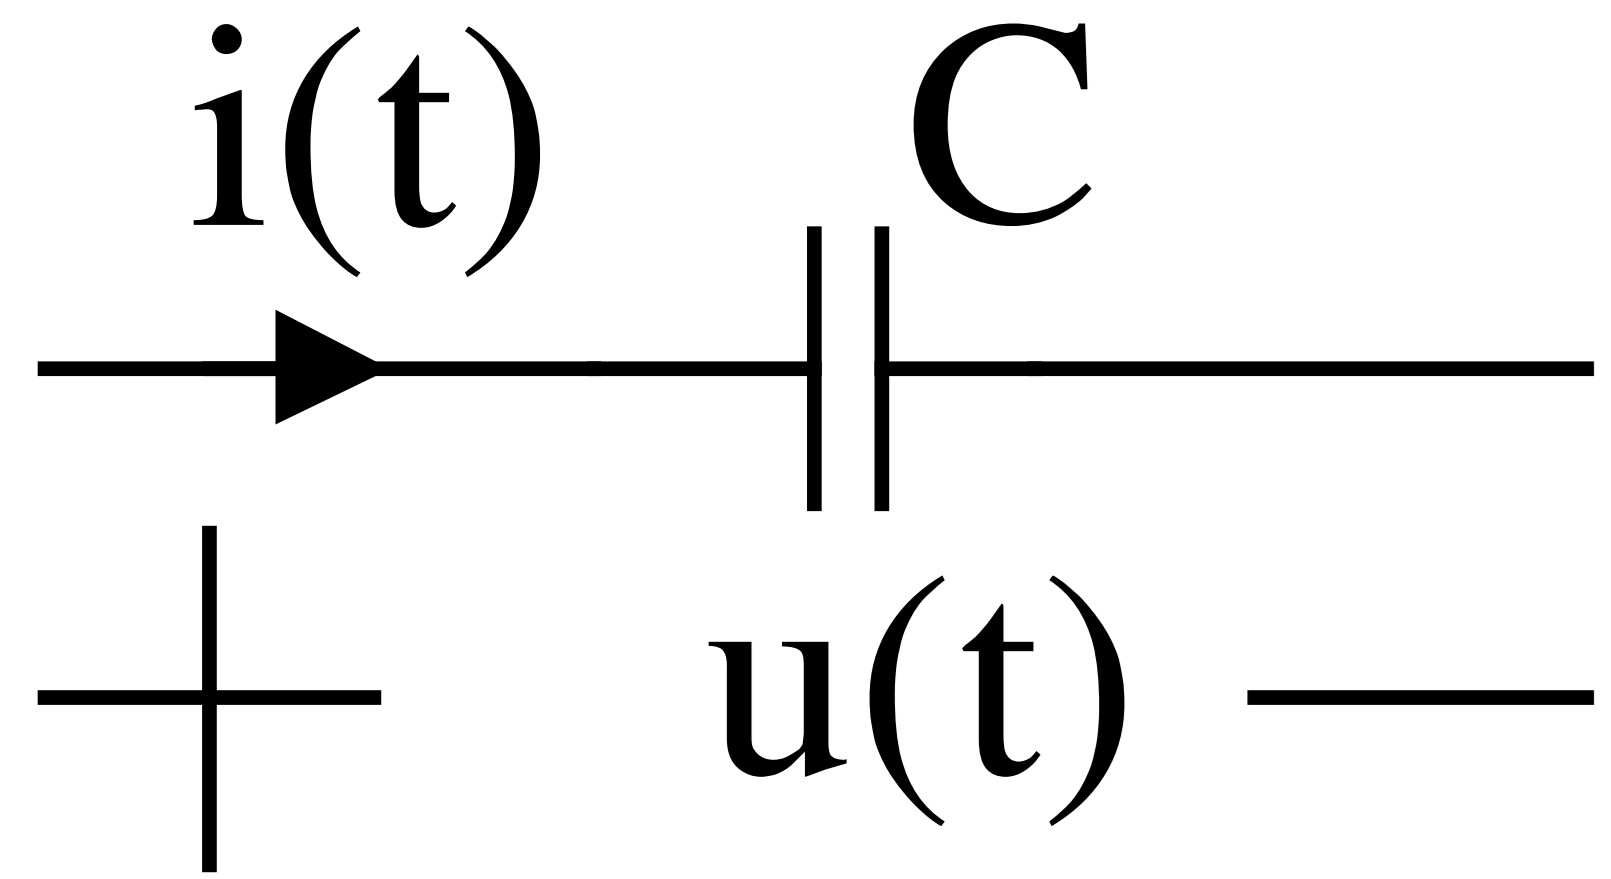
\includegraphics[width = 0.3\textwidth]{./image/51.png} \qquad 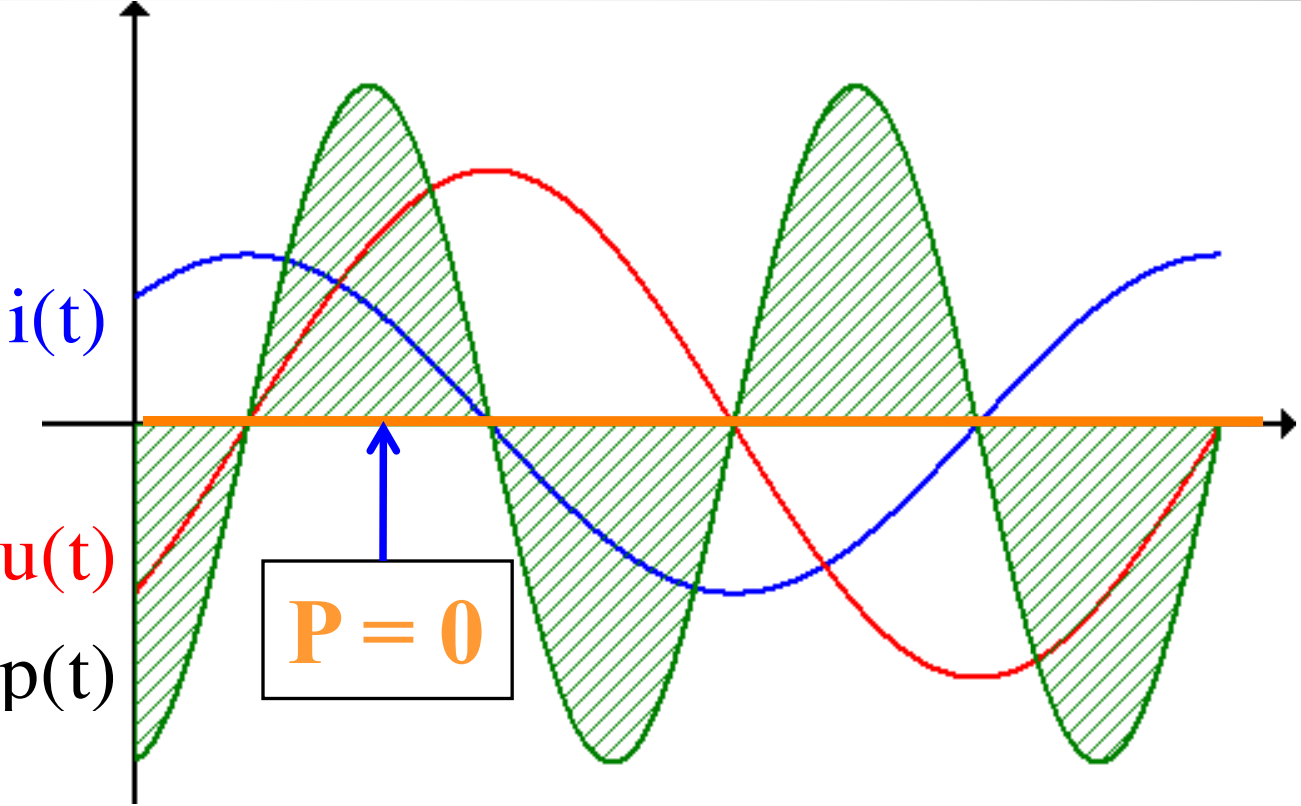
\includegraphics[width = 0.5\textwidth]{./image/52.png}
\end{center}
\begin{equation}
    i = I_m \cos (\Omega t + \varPsi),\ u = \frac{1}{C}\int idt
\end{equation}
\begin{equation}
    p(t) = u(t)i(t) =\frac{i}{C}\int idt = \frac{1}{\omega C}I^2_m \cos (\omega t + \varPsi) \sin (\omega t + \varPsi) = -\frac{1}{2}X_C I^2_m \sin (2\omega t + 2\varPsi) 
\end{equation}
\begin{empheq}[box=\widefbox]{align}
    P &= 0 \\
    Q &= \frac{-1}{2\omega C} I^2_m \\
    Q &= \frac{-1}{\omega C} I^2
\end{empheq}
\subsubsection{Công suất biểu kiến (Apparent Power)}
Định nghĩa: \begin{equation}
    S=UI=\frac{1}{2}U_mI_m \ \lbrack VA \rbrack
\end{equation}
Các cách tính khác:
\begin{equation}
    \begin{aligned}
        P &= UI\cos \varphi \\
        Q &= UI\sin \varphi \\
        S &= \sqrt{P^2 + Q^2}
    \end{aligned} \qquad
    \vcenter{\hbox{\begin{minipage}{5cm}
        \centering
        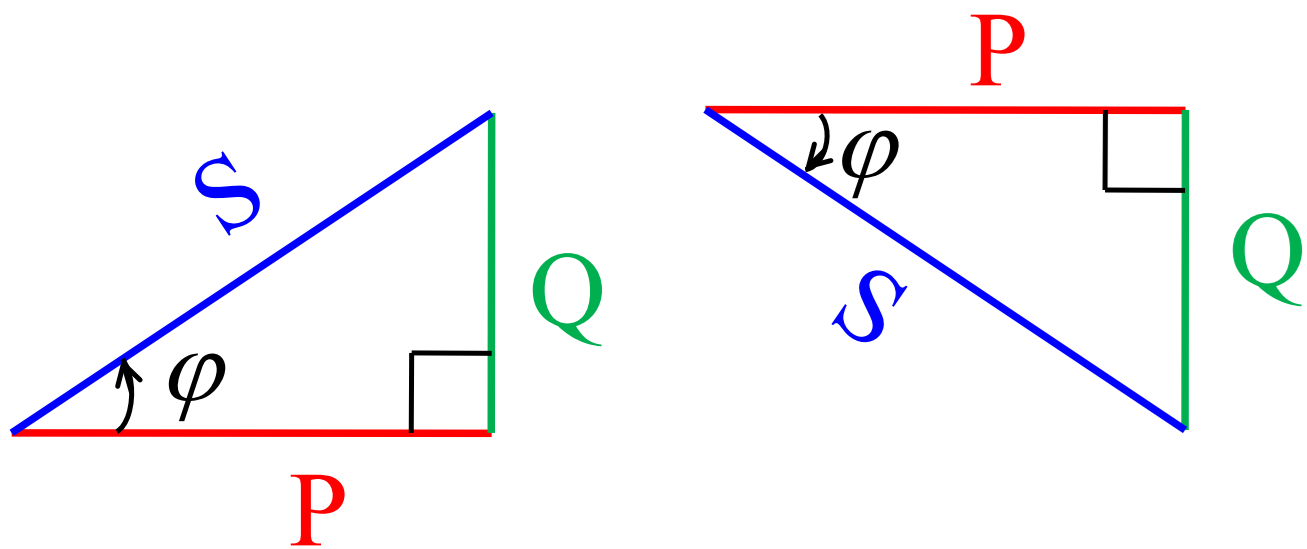
\includegraphics[width = 1.5\textwidth]{./image/53.png}
        \end{minipage}}}
\end{equation}
Công suất phức
\begin{equation}
    \tilde{S} = \frac{1}{2}\dot{U}_m I^*_m = \dot{U} I^* \ \lbrack VA \rbrack
\end{equation}
\begin{equation}
    \begin{aligned}
        P &= \text{Re} \lbrace \tilde{S} \rbrace \\
        Q &= \text{Im} \lbrace \tilde{S} \rbrace
    \end{aligned}
\end{equation}
\subsubsection{Nguyên lý cân bằng công suất}
\begin{equation}
    \sum P_{send} = \sum P_{receive} \Leftrightarrow \sum EI_E \cos \varphi_E + \sum JU_J \cos \varphi_J = \sum RI^2_R
\end{equation}
\begin{equation}
    \sum Q_{send} = \sum Q_{receive} \Leftrightarrow \sum EI_E \sin \varphi_E + \sum JU_J \sin \varphi_J = \sum XI^2_X
\end{equation}
\begin{equation}
    \begin{aligned}
        \Rightarrow \sum \tilde{S}_{send} &= \sum \tilde{S}_{receive} \\
        \sum \dot{E} I^*_E + \sum \dot{U}_J J^* &= \sum RI^2_R + \sum XI^2_X
    \end{aligned}
\end{equation}
\subsection{Hệ số công suất và cách hiệu chỉnh}
Hệ số công suất: $\cos \varphi = \dfrac{P}{S}$
\begin{itemize}
    \item $\cos \varphi$ sớm, vượt: nhánh dung $\varphi < 0$.
\end{itemize}
\begin{center}
    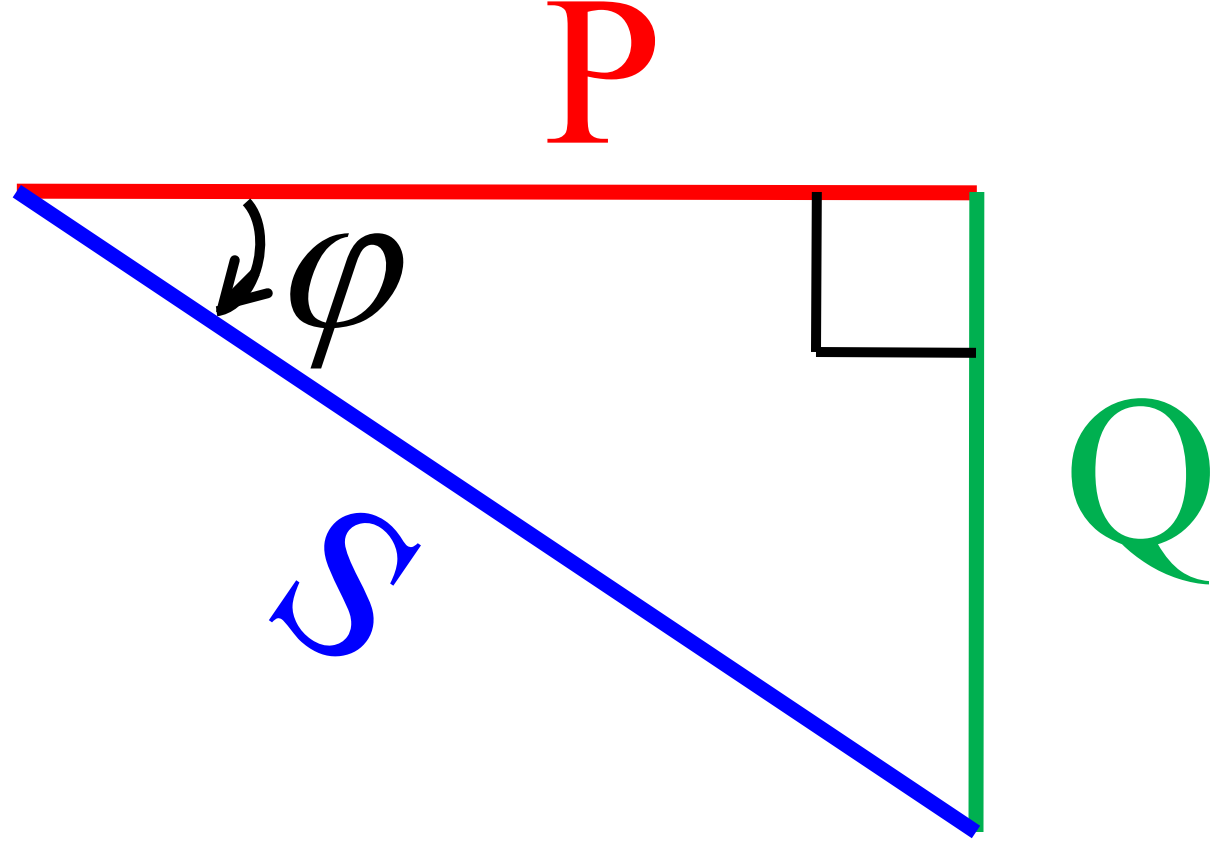
\includegraphics[width = 0.2\textwidth]{./image/54.png}
\end{center}
\begin{itemize}
    \item $\cos \varphi$ trễ, chậm: nhánh cảm $\varphi > 0$.
\end{itemize}
\begin{center}
    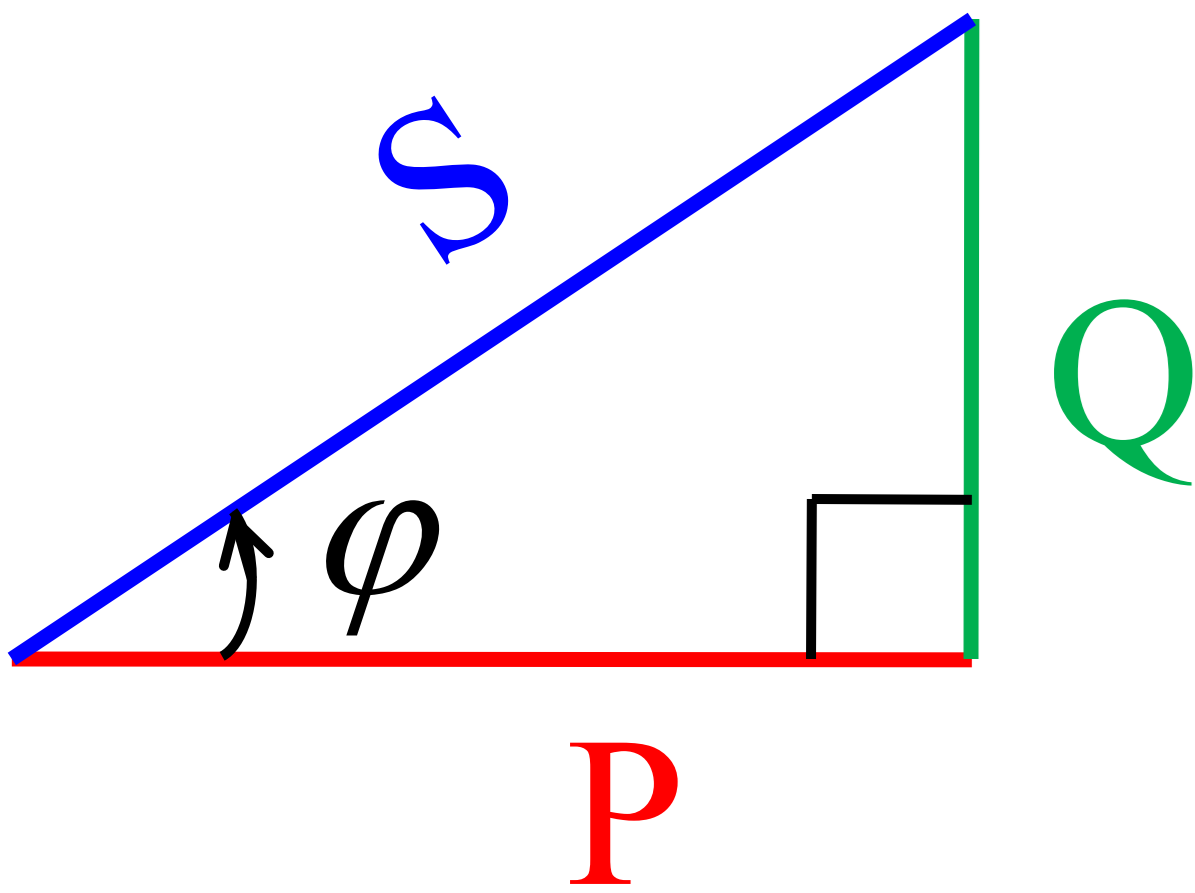
\includegraphics[width = 0.2\textwidth]{./image/55.png}
\end{center}
\subsubsection{Hiệu chỉnh hệ số công suất}
\begin{center}
    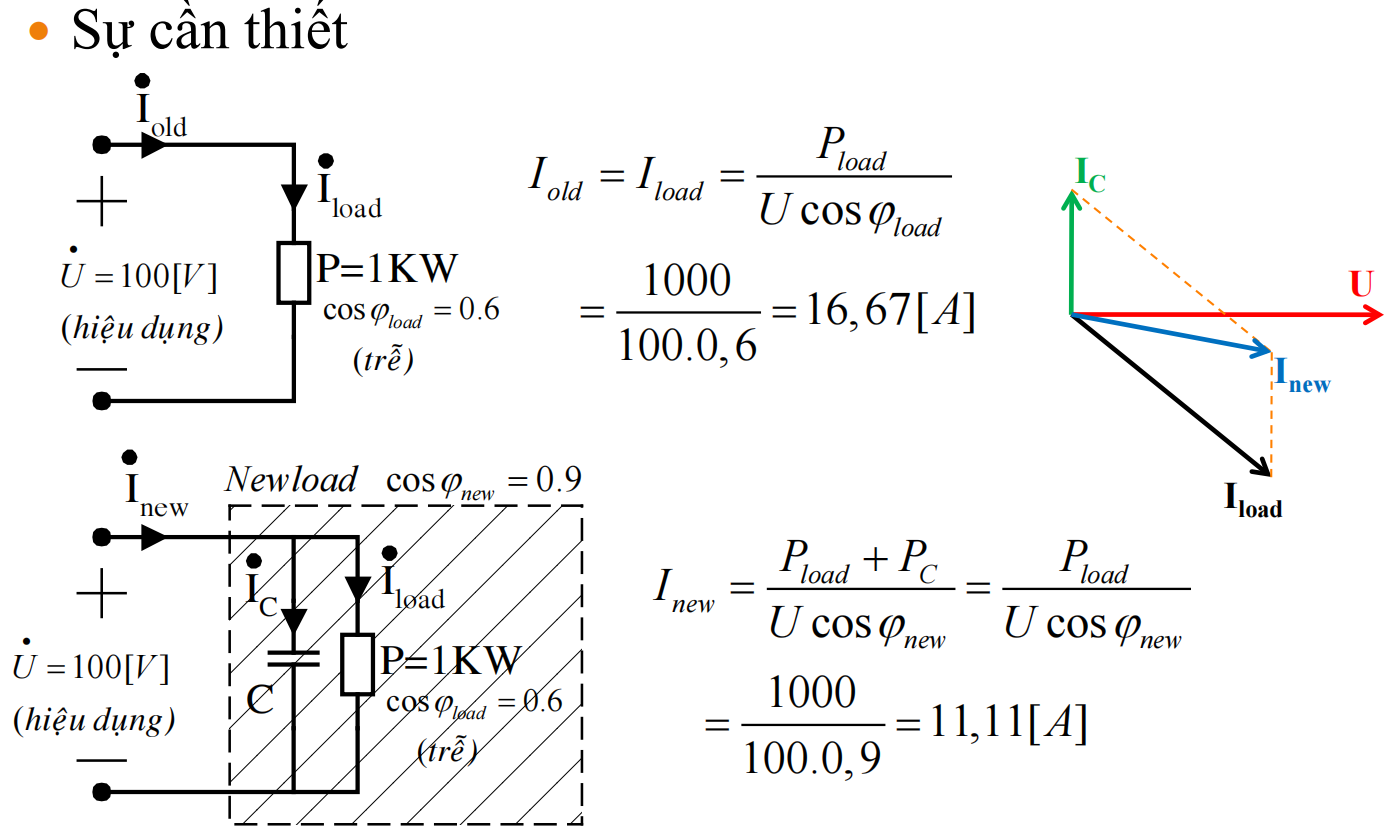
\includegraphics[width = 0.9\textwidth]{./image/56.png}
\end{center}
- Tải ban đầu

\begin{equation}
    \tilde{S}_{\text {old }}=P_{\text {old }}+j Q_{\text {old }} \rightarrow Q_{\text {old }}=P_{\text {old }} \operatorname{tg} \varphi_{\text {old }}
\end{equation}
- Sau hiệu chỉnh, thêm vào điện kháng $X$ đối nghịch tính tải \begin{equation}
    P_{\text {new }}=P_{\text {old }}+P_X=P_{\text {old }} \Longrightarrow Q_{\text {new }}=P_{\text {old }} \operatorname{tg}\left( \pm \arccos \varphi_{\text {new }}\right)
\end{equation}
\begin{equation}
    \Delta Q=Q_{\text {new }}-Q_{\text {old }}
\end{equation}
- Phần tử kháng cần
\begin{equation}
    L=\frac{U^2}{\omega \Delta Q} \ [H]
\end{equation}

cho hiệu chỉnh
\begin{equation}
    C=\frac{-\Delta Q}{\omega U^2} \ [F]
\end{equation}
\subsubsection{Đo công suất}
Watt kế:
\begin{itemize}
    \item Nội trở cuộn dòng điện: $R_{11} \approx 0$
    \item Nội trở cuộn điện áp: $R_{22} \approx \infty$
    \item Cực cùng tên: $\ast, \pm, \bullet$ (giúp xác định hướng truyền công suất)
\end{itemize}
\begin{center}
    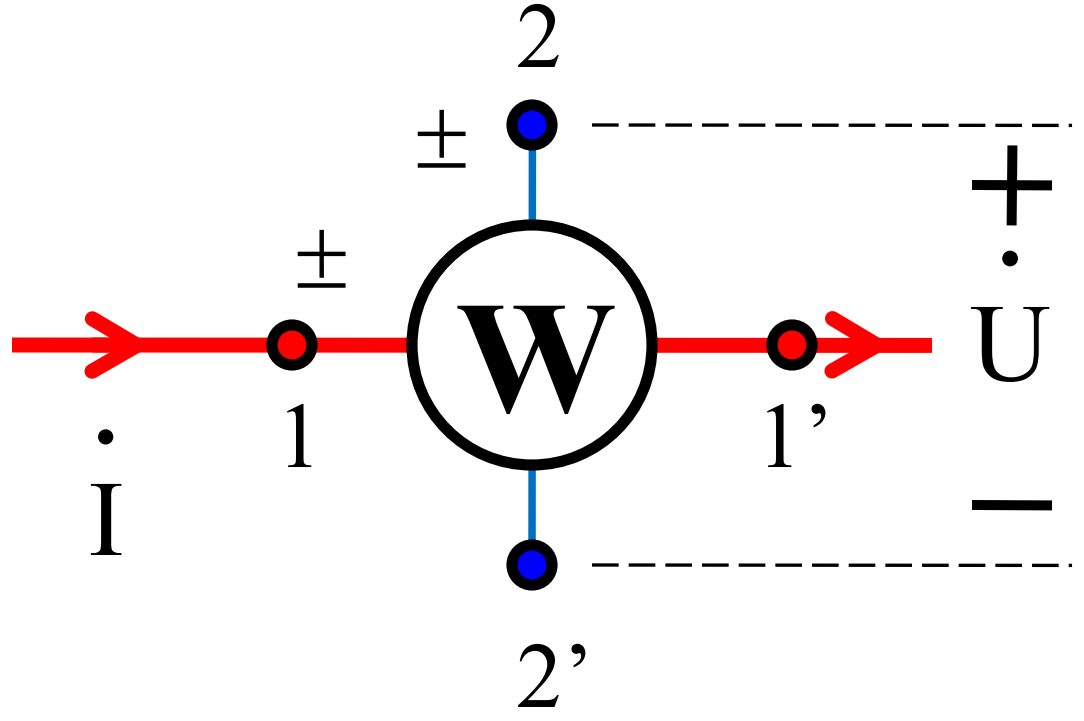
\includegraphics[width = 0.5\textwidth]{./image/57.png}
\end{center}
Số chỉ:
\begin{equation}
    \begin{aligned}
        P &= \frac{1}{2}U_m I_m\cos(\varphi_u - \varphi_i) = UI\cos (\varphi_u - \varphi_i) \\
          &= \frac{1}{2} \text{Re} \lbrace \dot{U}_m I^*_m \rbrace = \text{Re} \lbrace \dot{U} I^* \rbrace
    \end{aligned}
\end{equation}
\subsection{Phối hợp trở kháng}
\subsection{Mạch cộng hưởng}
\textbf{\textul{Phần tử thực}}

Cuộn dây luôn có điện trở dây quấn.
\begin{center}
    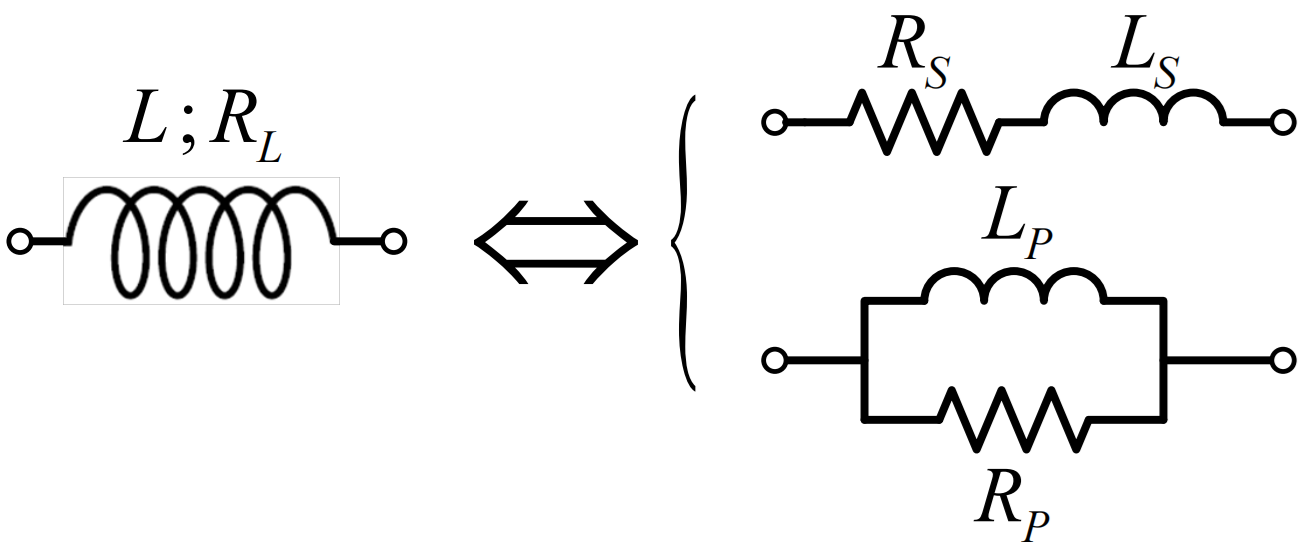
\includegraphics[width = 0.6\textwidth]{./image/59.png}
\end{center}

Tụ điện luôn có điện trở rò rỉ.
\begin{center}
    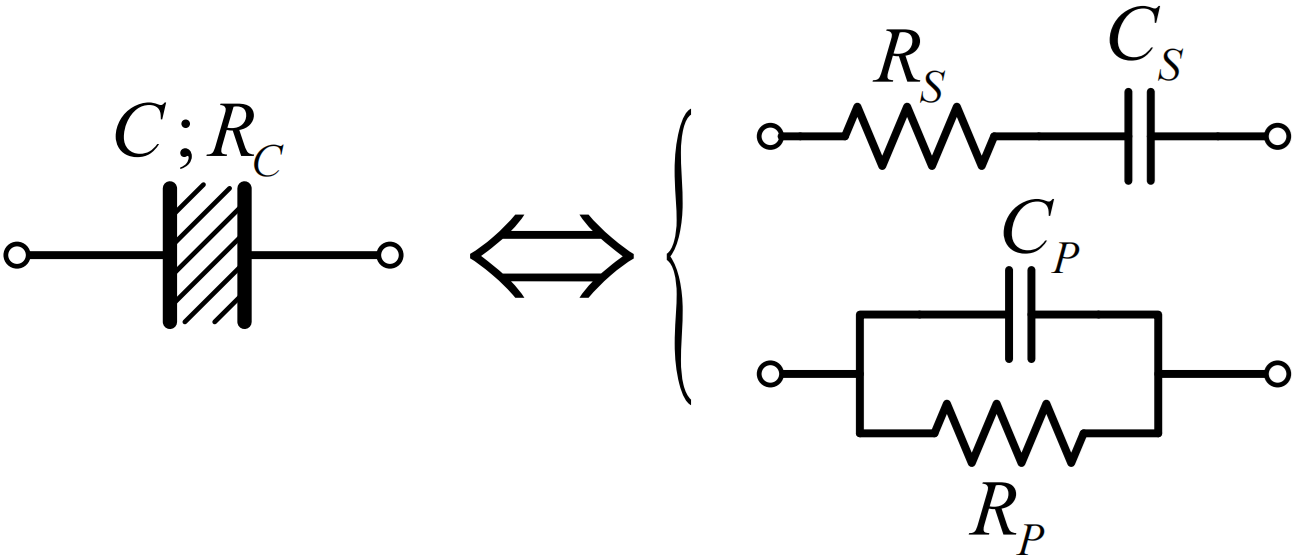
\includegraphics[width = 0.6\textwidth]{./image/60.png}
\end{center}

\textbf{\textul{Qui đổi tương đương}}

Cuộn dây: 
\begin{equation}
    \vcenter{\hbox{\begin{minipage}{4cm}
        \centering
        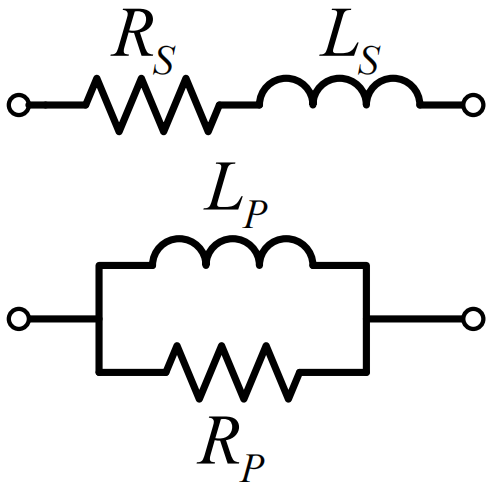
\includegraphics[width = 0.8\textwidth]{./image/61.png}
        \end{minipage}}}
    \left.
        \begin{aligned}
            Z_S &= R_S + j\omega L_S \\
            Y_P &= \dfrac{1}{R_P} - j\dfrac{1}{\omega L_P}
        \end{aligned}
    \right\} \to 
    \left\{
        \begin {aligned}
            Z_S &= \dfrac{1}{Y_P} = \dfrac{\omega^2 L^2_P R_P + j\omega L_P R^2_P}{R^2_P + \omega^2 L^2_P} \\
            Y_P &= \dfrac{1}{Z_S} = \dfrac{R_S + j\omega L_S}{R^2_S + \omega^2 L^2_S}
        \end{aligned}
    \right.
\end{equation}

Tụ điện:
\begin{equation}
    \vcenter{\hbox{\begin{minipage}{4cm}
        \centering
        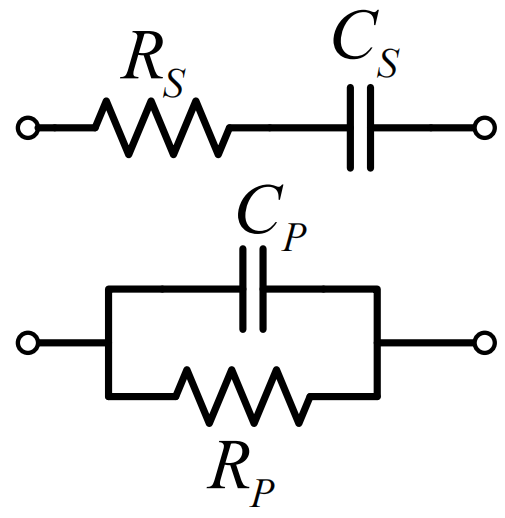
\includegraphics[width = 0.8\textwidth]{./image/62.png}
        \end{minipage}}}
    \left.
        \begin{aligned}
            Z_S &= R_S - \dfrac{j}{\omega C_S} \\
            Y_P &= \dfrac{1}{R_P} + j\omega C_P
        \end{aligned}
    \right\} \to 
    \left\{
        \begin {aligned}
            Z_S &= \dfrac{1}{Y_P} = \dfrac{R_P - j\omega C_P R^2_P}{1 + \omega^2 C^2_P R^2_P} \\
            Y_P &= \dfrac{1}{Z_S} = \dfrac{\omega^2 C^2_S R_S + j\omega C_S}{1 + \omega^2 C^2_S R^2_S}
        \end{aligned}
    \right.
\end{equation}

$\divideontimes$ Hệ số phẩm chất:
\begin{equation}
    Q = 2\pi \frac{W_{\max}}{W_T}
\end{equation}

$W_{\max}:$ năng lượng tích lũy max.

$W_T:$ năng lượng tiêu tán trong 1 chu kỳ.

$\divideontimes$ Hệ số tổn hao:
\begin{equation}
    D=tg \delta
\end{equation}

$\delta:$ góc mất (tổn hao).

Quan hệ D $\&$ Q: 
\begin{equation}
    D.Q=1
\end{equation}

\textbf{\textul{Qui đổi tương đương}}

Cuộn dây:
\begin{equation}
    Q = \frac{\omega L_S}{R_S} = \frac{R_P}{\omega L_P}
\end{equation}
\begin{equation}
    \left.
        \begin{aligned}
            Z_S &= \frac{1}{Y_P} = \frac{1}{1+Q^2}(R_P + j\omega L_P Q^2) \\
            Y_P &= \frac{1}{Z_S} = \frac{1}{1+Q^2}\left(\frac{1}{R_S} - j\frac{Q^2}{\omega L_S}\right)
        \end{aligned}
    \right\} \to 
    \left\{
        \begin {aligned}
            (1+Q^2) R_S = R_P \\
            \left( 1 + \frac{1}{Q^2} \right)L_S = L_P
        \end{aligned}
    \right.
\end{equation}

Tụ điện:
\begin{equation}
    D = \omega C_S R_S = \frac{1}{\omega C_P R_P}
\end{equation}
\begin{equation}
    \left.
        \begin{aligned}
            Z_S &= \frac{1}{1+D^2}\left(D^2 R_P - j\frac{1}{\omega C_P} \right) \\
            Y_P &= \frac{1}{1+D^2}\left(\frac{D^2}{R_S} + j\omega C_S\right)
        \end{aligned}
    \right\} \to 
    \left\{
        \begin {aligned}
            \left(1+\frac{1}{D^2} \right) R_S = R_P \\
            \frac{1}{1+D^2} C_S = C_P
        \end{aligned}
    \right.
\end{equation}

\textul{\textbf{Hiện tượng cộng hưởng nhánh:}}

Trên một nhánh nối tiếp hoặc song song khi dòng và áp cùng pha ta có cộng hưởng.

Từ $\dot{U} =Z\dot{I} \ \& \ \dot{I} = Y\dot{U} \Rightarrow$ Z hay Y: số thực
\begin{center}
    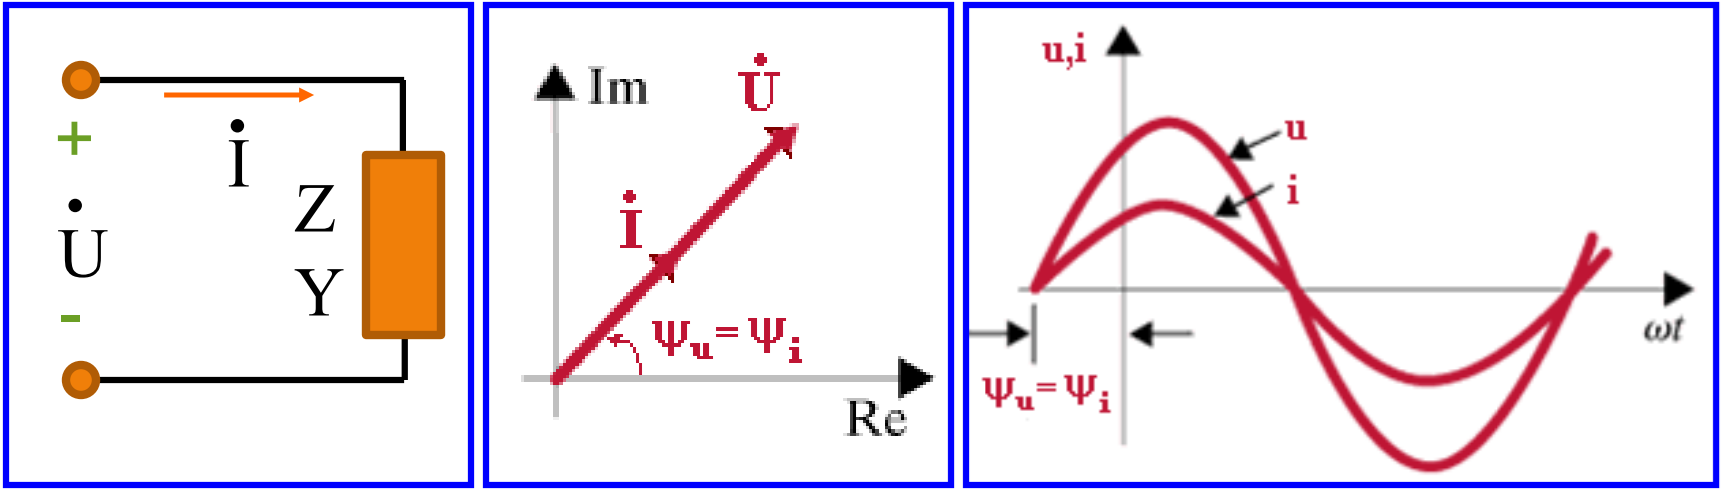
\includegraphics[width = 1\textwidth]{./image/63.png}
\end{center}
\begin{itemize}
    \item Z thực: cộng hưởng nối tiếp.
    \item Y thực: cộng hưởng song song.
\end{itemize}
\subsubsection{Mạch cộng hưởng nối tiếp}
$\divideontimes$ Mạch RLC nối tiếp: áp vào $u(t)$ có biên độ $U_m$ cố định, tần số $\omega$ thay đổi được.
\begin{center}
    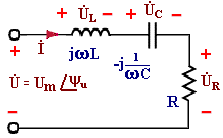
\includegraphics[width = 0.5\textwidth]{./image/64.png}
\end{center}
Trở kháng nhánh:
\begin{equation}
    \begin{aligned}
        Z &= R + j\left(\omega L - \frac{1}{\omega C}\right) \\
        \Rightarrow |Z| &= \sqrt{R^2 + \left(\omega L - \frac{1}{\omega C}\right)^2} \\
        \Rightarrow \text{Im} \lbrace Z \rbrace &= \omega L - \frac{1}{\omega C}
    \end{aligned}
\end{equation}
Trở kháng nhánh thay đổi theo tần số $\omega$.
\begin{center}
    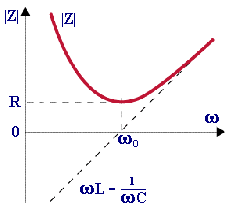
\includegraphics[width = 0.3\textwidth]{./image/65.png}
\end{center}

\textbf{$\divideontimes$ Tần số cộng hưởng nối tiếp:} Là tần số $\omega_0$ thỏa:
\begin{equation}
    \text{Im} \lbrace Z(\omega_0) \rbrace = \omega L - \frac{1}{\omega C} = 0
    \qquad \vcenter{\hbox{\begin{minipage}{5cm}
        \centering
        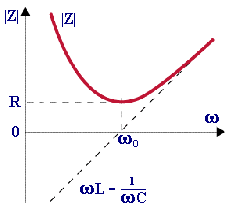
\includegraphics[width = 1\textwidth]{./image/66.png}
        \end{minipage}}}
\end{equation}

Tại tần số cộng hưởng: $|Z| \to \min = R$ và nhánh thuần trở.

\textbf{$\divideontimes$ Băng thông (BW) của mạch cộng hưởng:}
\begin{itemize}
    \item Dòng qua nhánh $\leftrightsquigarrow$ áp trên R, có module:
        \begin{equation}
            U_R = U_m \frac{R}{\sqrt{R^2 + \left(\omega L - \dfrac{1}{\omega C}\right)^2}} \Rightarrow U_{R(\max)} = U_m
        \end{equation}
    \item Tần số cắt khi:
        \begin{equation}
            U_R = \frac{1}{\sqrt{2}}U_{R(\max)} \qquad \vcenter{\hbox{\begin{minipage}{6cm}
                \centering
                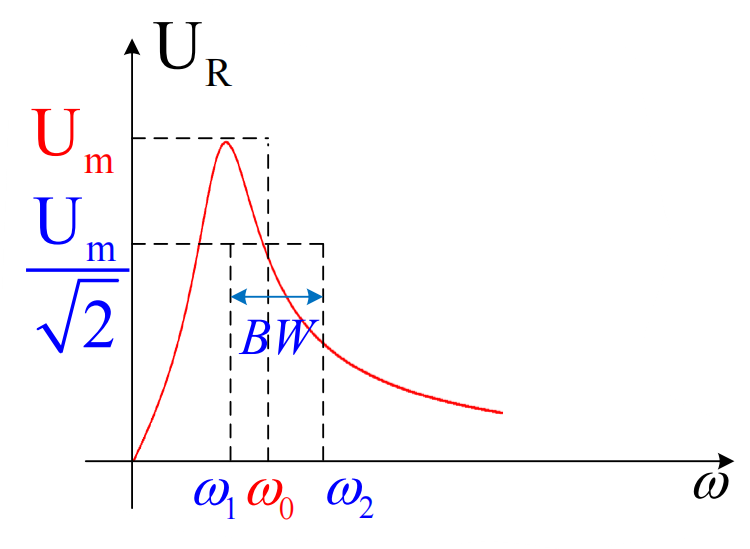
\includegraphics[width = 1\textwidth]{./image/67.png}
                \end{minipage}}}
        \end{equation}
    \item Băng thông: $BW = \omega_2 - \omega_1$ hay $BW = f_2 - f_1 \ $ Hz.
\end{itemize}

\textbf{$\divideontimes$ Xác định tần số cắt:}
\begin{center}
    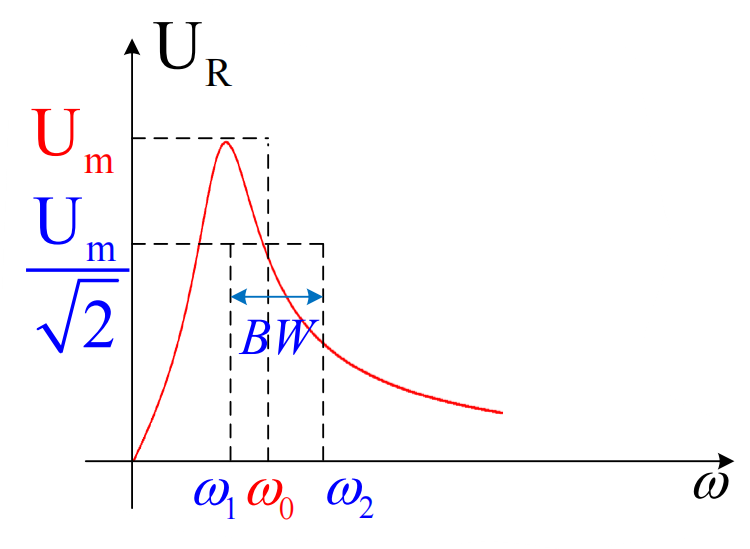
\includegraphics[width = 0.5\textwidth]{./image/67.png}
\end{center}
\begin{equation}
    U_{R(\omega_1 \ \& \ \omega_2)} = U_m \frac{R}{\sqrt{R^2 + \left(\omega L - \dfrac{1}{\omega C}\right)^2}} = \frac{U_m}{\sqrt{2}}
\end{equation}
\begin{equation}
    \omega_1 = -\frac{R}{2L} + \sqrt{\left( \frac{R}{2L} \right)^2 + \frac{1}{LC}} \qquad \omega_2 = \frac{R}{2L} + \sqrt{\left( \frac{R}{2L} \right)^2 + \frac{1}{LC}}
\end{equation}
\begin{equation}
    BW = \frac{R}{L} \ \lbrack rad/s \rbrack
\end{equation}

\textbf{$\divideontimes$ Hệ số phẩm chất:}
\begin{equation*}
    Q = 2\pi \frac{W_{\max}}{W_T}
\end{equation*}
Ở mạch cổng hưởng nối tiếp, người ta chứng minh được:
\begin{equation}
    \begin{aligned}
        W_{\max} &= \max (W_L + W_C) = const = \frac{1}{2}LI^2_m \\
        W_T &= \frac{1}{2}RI^2_m T = \frac{1}{2}RI^2_m \frac{2\pi}{\omega_0} \\
        \Rightarrow Q &= \frac{\omega_0 L}{R} = \frac{1}{\omega_0 RC} = \frac{\omega_0}{BW}
    \end{aligned}
\end{equation}

%\textbf{$\divideontimes$ Tính tần số cắt theo hệ số phẩm chất:}
\textbf{$\divideontimes$ Đồ thị vecotr tại cộng hưởng:}
Do: $U_{Lm} = U_{Cm} = \omega_0 LI_m = \frac{I_m}{\omega_0 C}$
\begin{equation}
    \frac{U_{Lm}}{U_m} = \frac{U_{Cm}}{U_m} = \frac{\omega_0 LI_m}{RI_m} = \frac{\omega_0 L}{R} = Q
    \qquad \vcenter{\hbox{\begin{minipage}{5cm}
        \centering
        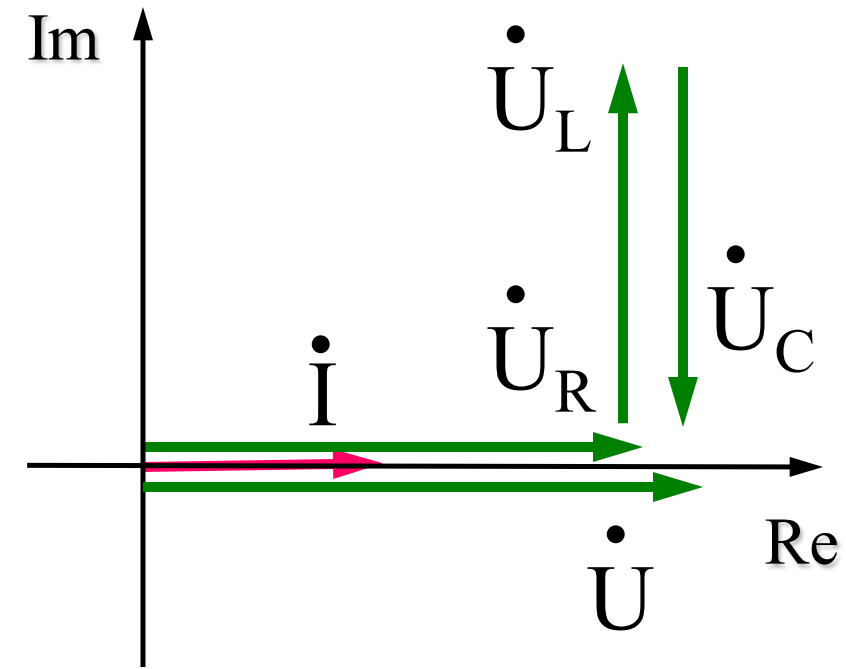
\includegraphics[width = 1\textwidth]{./image/68.png}
        \end{minipage}}}
\end{equation}
Cộng hưởng nối tiếp gọi là cộng hưởng áp vì tại lân cận tần số cộng hưởng, áp trên các phần tử kháng rất lớn so với tín hiệu áp vào của mạch (Q lần).

\begin{equation*}
    \vcenter{\hbox{\begin{minipage}{8cm}
        \centering
        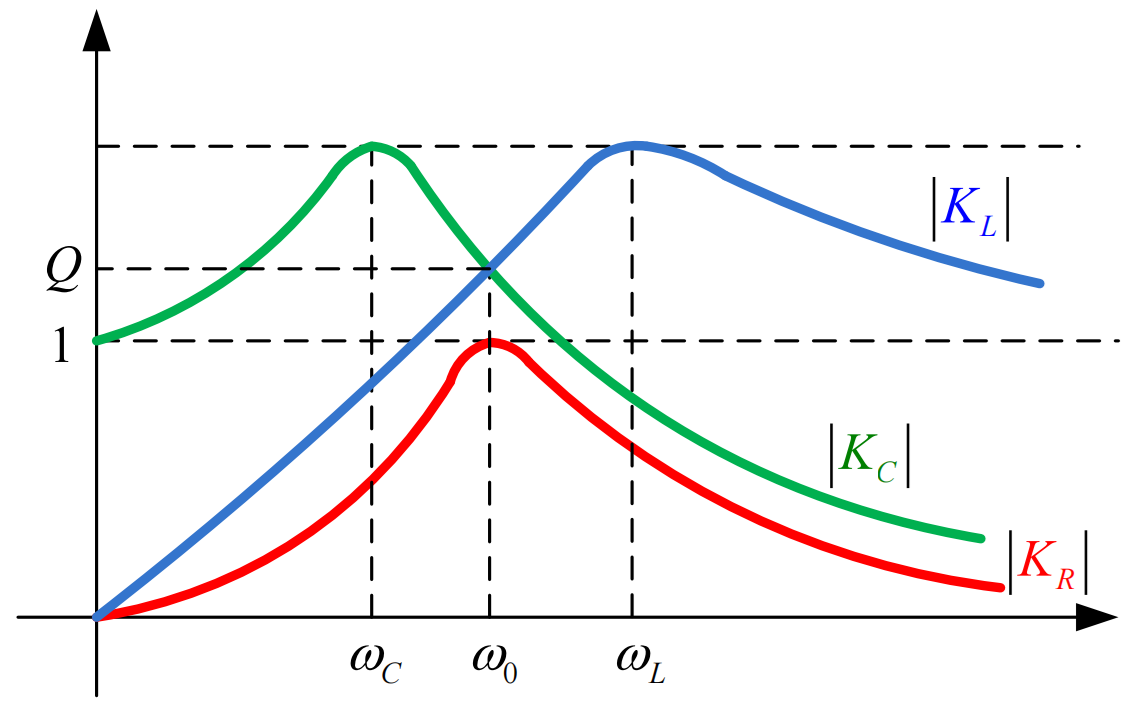
\includegraphics[width = 1\textwidth]{./image/69.png}
        \end{minipage}}} 
    \qquad Q > \frac{1}{\sqrt{2}}
\end{equation*}
\begin{equation*}
    \vcenter{\hbox{\begin{minipage}{8cm}
        \centering
        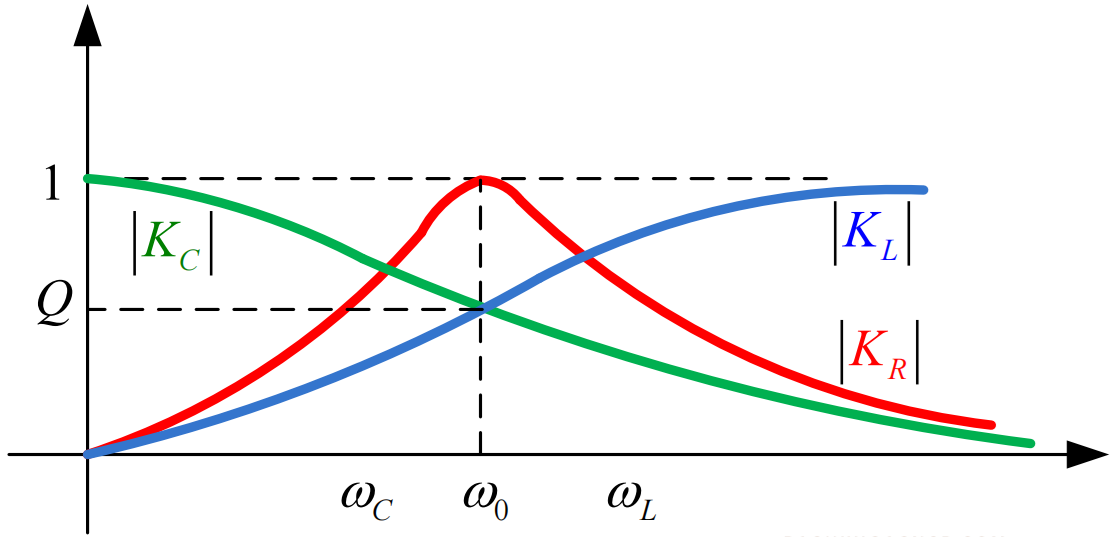
\includegraphics[width = 1\textwidth]{./image/70.png}
        \end{minipage}}} 
    \qquad Q < \frac{1}{\sqrt{2}}
\end{equation*}
\subsubsection{Mạch cộng hưởng song song}
$\divideontimes$ Mạch RLC song song: dòng vào $J(t)$ có biên độ cố định $J_m$, tần số $\omega$ thay đổi được.
\begin{center}
    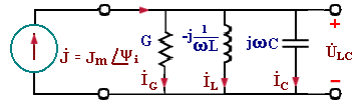
\includegraphics[width = 0.5\textwidth]{./image/71.png}
\end{center}
Dẫn nạp nhánh:
\begin{equation}
    \begin{aligned}
        Y &= G + j\left(\omega C - \frac{1}{\omega L}\right) \\
        \Rightarrow |Y| &= \sqrt{G^2 + \left(\omega C - \frac{1}{\omega L}\right)^2} \\
        \Rightarrow \text{Im} \lbrace Y \rbrace &= \omega C - \frac{1}{\omega L}
    \end{aligned}
\end{equation}
Dẫn nạp nhánh thay đổi theo tần số $\omega$.
\begin{center}
    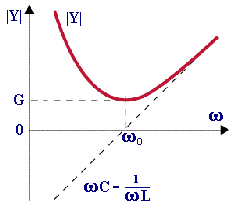
\includegraphics[width = 0.3\textwidth]{./image/72.png}
\end{center}

\textbf{$\divideontimes$ Tần số cộng hưởng song song:} Là tần số $\omega_0$ thỏa:
\begin{equation}
    \text{Im} \lbrace y(\omega_0) \rbrace = \omega C - \frac{1}{\omega L} = 0
    \qquad \vcenter{\hbox{\begin{minipage}{5cm}
        \centering
        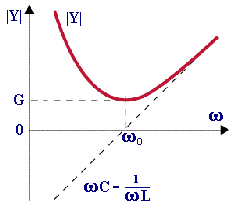
\includegraphics[width = 1\textwidth]{./image/72.png}
        \end{minipage}}}
\end{equation}

Tại tần số cộng hưởng: $|Y| \to \min = G$ và nhánh thuần trở.

\textbf{$\divideontimes$ Băng thông (BW) của mạch cộng hưởng:}
\begin{itemize}
    \item Áp trên nhánh $\leftrightsquigarrow$ áp trên khung LC, có module:
        \begin{equation}
            U_{LC} = \frac{J_m}{\sqrt{G^2 + \left(\omega C - \dfrac{1}{\omega L}\right)^2}} \Rightarrow U_{LC(\max)} = \frac{J_m}{G}
        \end{equation}
    \item Tần số cắt khi:
        \begin{equation}
            U_{LC} = \frac{1}{\sqrt{2}}U_{LC(\max)} \qquad \vcenter{\hbox{\begin{minipage}{6cm}
                \centering
                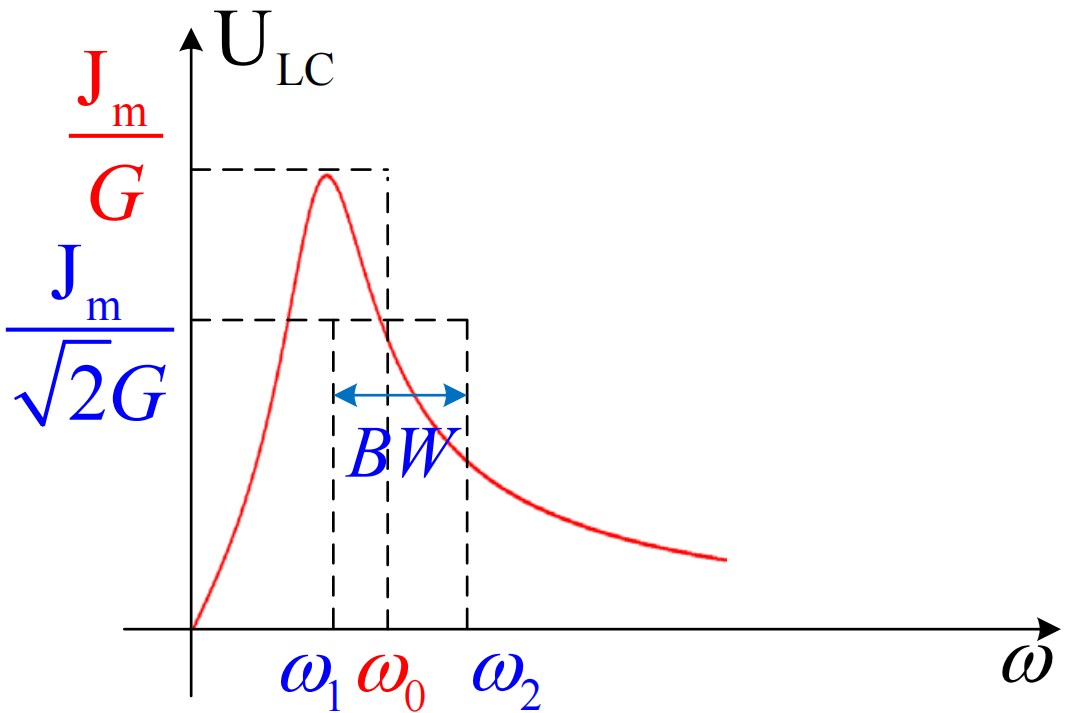
\includegraphics[width = 1\textwidth]{./image/73.png}
                \end{minipage}}}
        \end{equation}
    \item Băng thông: $BW = \omega_2 - \omega_1$ hay $BW = f_2 - f_1 \ $ Hz.
\end{itemize}

\textbf{$\divideontimes$ Xác định tần số cắt:}
\begin{center}
    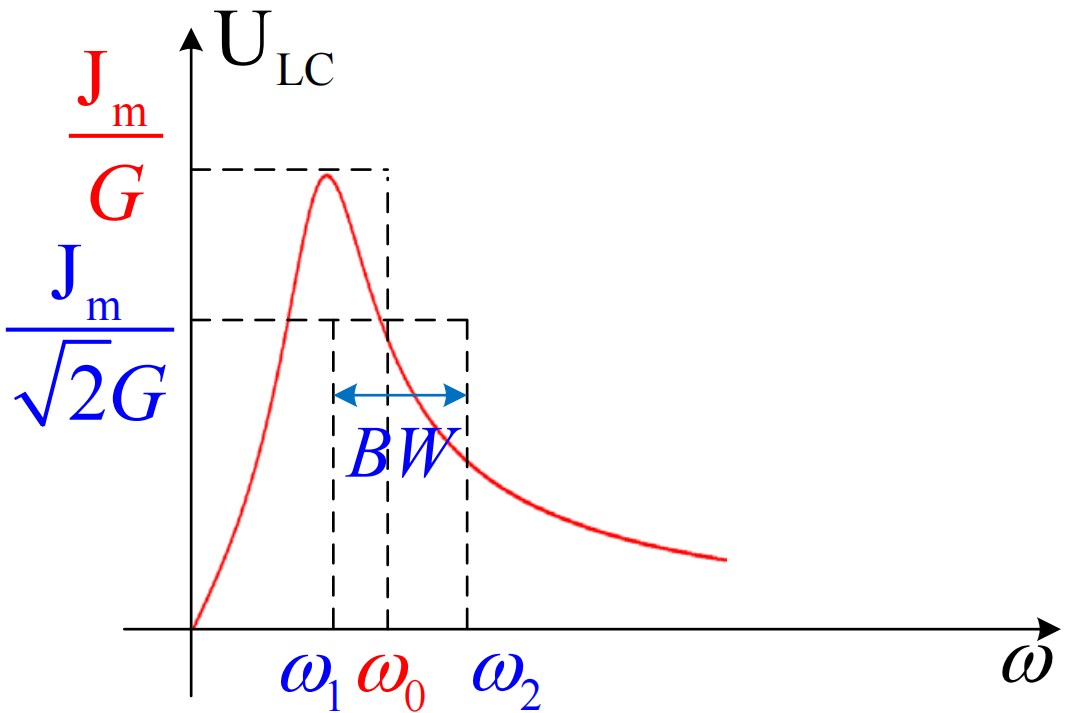
\includegraphics[width = 0.5\textwidth]{./image/73.png}
\end{center}
\begin{equation}
    U_{LC(\omega_1 \ \& \ \omega_2)} = \frac{J_m}{\sqrt{G^2 + \left(\omega C - \dfrac{1}{\omega L}\right)^2}} = \frac{J_m}{\sqrt{2}G}
\end{equation}
\begin{equation}
    \omega_1 = -\frac{G}{2C} + \sqrt{\left( \frac{G}{2C} \right)^2 + \frac{1}{LC}} \qquad \omega_2 = \frac{G}{2C} + \sqrt{\left( \frac{G}{2C} \right)^2 + \frac{1}{LC}}
\end{equation}
\begin{equation}
    BW = \frac{G}{C} \ \lbrack rad/s \rbrack
\end{equation}

\textbf{$\divideontimes$ Hệ số phẩm chất:}
\begin{equation*}
    Q = 2\pi \frac{W_{\max}}{W_T}
\end{equation*}
Ở mạch cổng hưởng nối tiếp, người ta chứng minh được:
\begin{equation}
    \begin{aligned}
        W_{\max} &= \max (W_L + W_C) = const = \frac{1}{2}CU^2_{LCm} \\
        W_T &= \frac{1}{2}GU^2_{LCm} T = \frac{1}{2}GU^2_{LCm} \frac{2\pi}{\omega_0} \\
        \Rightarrow Q &= \frac{\omega_0 C}{G} = \frac{1}{\omega_0 LG} = \frac{\omega_0}{BW}
    \end{aligned}
\end{equation}

\textbf{$\divideontimes$ Đồ thị vecotr tại cộng hưởng:}
Do: $I_{Lm} = I_{Cm} = \omega_0 CU_{LCm} = \frac{U_{LCm}}{\omega_0 L}$
\begin{equation}
    \frac{I_{Lm}}{J_m} = \frac{I_{Cm}}{J_m} = \frac{\omega_0 CU_{LCm}}{GU_{LCm}} = \frac{\omega_0 C}{G} = Q
    \qquad \vcenter{\hbox{\begin{minipage}{5cm}
        \centering
        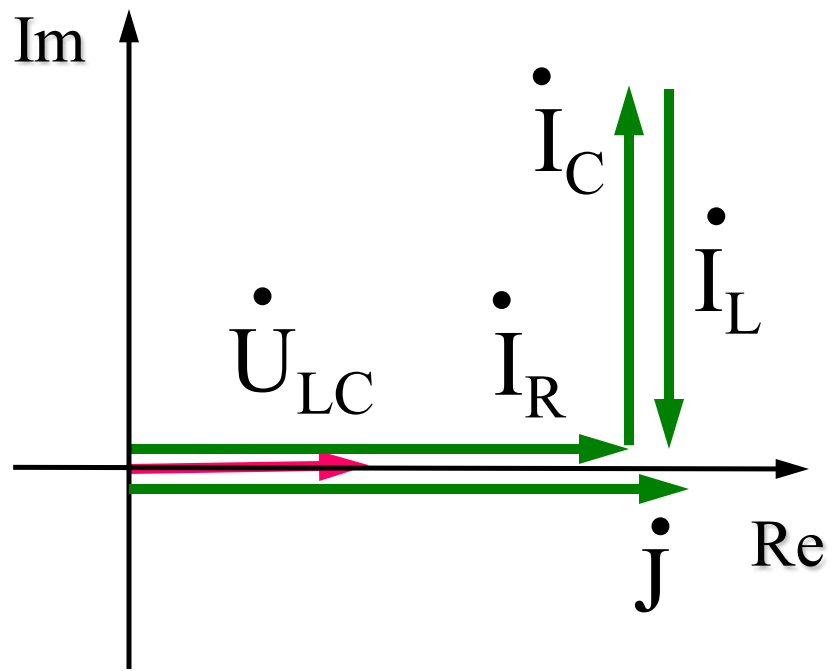
\includegraphics[width = 1\textwidth]{./image/74.png}
        \end{minipage}}}
\end{equation}
Cộng hưởng song song gọi là cộng hưởng dòng vì tại lân cận tần số cộng hưởng, biên độ dòng qua các phần tử kháng rất lớn so với biên độ tín hiệu dòng đưa vào mạch (Q lần).
